\documentclass{article}

\PassOptionsToPackage{numbers,sort&compress}{natbib}
\usepackage[main]{neurips_2026}

\usepackage[utf8]{inputenc}
\usepackage[T1]{fontenc}
\usepackage[hidelinks]{hyperref}
\usepackage{url}
\usepackage{booktabs}
\usepackage{amsfonts}
\usepackage{amsmath}
\usepackage{amssymb}
\usepackage{amsthm}
\usepackage{xcolor}
\usepackage{graphicx}
\usepackage{multirow}

\newif\iftcolorboxavailable
\IfFileExists{tcolorbox.sty}{\usepackage{tcolorbox}\tcolorboxavailabletrue}{\tcolorboxavailablefalse}

\setlength{\textfloatsep}{8pt plus 1pt minus 2pt}
\setlength{\floatsep}{7pt plus 1pt minus 2pt}
\setlength{\intextsep}{7pt plus 1pt minus 2pt}
\setlength{\abovecaptionskip}{4pt}
\setlength{\belowcaptionskip}{0pt}

\title{Conformal Open-Vocabulary Detection: Hallucination FDR Control via Self-Normalized Betting e-Values}

\author{Anonymous Authors}

\newtheorem{lemma}{Lemma}
\newtheorem{theorem}{Theorem}
\newtheorem{corollary}{Corollary}
\newtheorem{proposition}{Proposition}
\theoremstyle{remark}
\newtheorem{remark}{Remark}

\newcommand{\IoU}{\mathrm{IoU}}
\newcommand{\FDR}{\mathrm{FDR}}
\newcommand{\E}{\mathbb{E}}
\newcommand{\Prob}{\mathbb{P}}
\newcommand{\1}{\mathbf{1}}
\newcommand{\R}{\mathcal{R}}
\newcommand{\Hnull}{\mathcal{H}_0}
\newcommand{\Halt}{\mathcal{H}_1}

\begin{document}

\maketitle

\begin{abstract}
Open-vocabulary detectors return high-confidence boxes for categories
that are not present: in a COCO absent-query pilot, the top-decile
detections are 100\% hallucinations. We show that, for category-name
or fixed-template prompts whose absence labels are auditable, post-hoc
false discovery rate (FDR) control is achievable on a frozen detector
by applying e-BH with self-normalized conformal betting e-values
within each image-query family, which tolerates the arbitrary
dependence induced by shared proposals and NMS. The power of this procedure is governed by a closed-form rejection
condition, which we call the \emph{activation frontier}. It is
necessary and sufficient, and is expressed in the family size, the
calibration pool aggregate, and the target level. The rejection
condition shows how family size, calibration evidence, and score
separation determine whether e-BH makes discoveries, and it
suggests practical variants such as score filtering, cluster-level
aggregation, and template-specific calibration. On COCO and
VOC with GroundingDINO, OWL-ViT, and YOLO-World, per-family FDP
stays below the nominal level at $\alpha=0.10$ across all six
configurations (max $1.7\%$) with recall $9.7$--$40.9\%$; a
stratified empirical Bernstein bound provides a non-vacuous pooled FDP
certificate ($\varepsilon\!=\!0.074$) on the 57\% of families with
$K\!\le\!5$; released detections on full COCO reach $93.6\%$ pooled
precision versus $72.9\%$ for p-value BH; cluster-level aggregation lifts
operational recall $1.7\times$ (COCO/GDino) and $5.8\times$
(RegionCLIP, no internal NMS). On LVIS and Open Images, observed
failures are consistent with the contamination mechanism identified
by the condition, which also indicates the bound under which
validity is restored.
\end{abstract}

\section{Introduction}
\label{sec:intro}

A binary conformal e-value that tests whether a detector score
exceeds a high calibration-null quantile is formally valid, yet in
our COCO pilot it rejects \emph{zero} detections despite the
top-decile being 100\% hallucinations (FDP $=1.0$) across
2{,}992 image-query families. The pilot points to quantization
rather than absence of signal: the e-value takes only two values,
while e-BH needs evidence that scales with family size. Looking at
the e-BH rejection condition directly, we call it the
\emph{activation frontier} (Theorem~\ref{thm:activation_frontier}):
in an image-query family of size $K$, e-BH rejects $r$ candidates
only if the $r$-th largest evidence exceeds
$K C_m / [\alpha r(m{+}1){-}K]$. The inequality is elementary but
will be used below to analyze power separately from validity, and
to trace three obstacles: detector-limited recall, non-exhaustive
annotations, and the failure of the natural fix that clips scores
to a high quantile.

Recent work documents the OVD hallucination problem~\cite{ruis2026fantastic},
yet detection-side reliability tools still focus on coverage and recall
rather than false discoveries. Standard Benjamini--Hochberg (BH)
procedures~\cite{benjamini1995controlling} require independence or PRDS
\cite{benjamini2001control}, assumptions that are difficult to justify
after proposal sharing and NMS. Existing conformal detection
tools~\cite{andeol:hal-05399935,silva2025conformal} do not target
family-level FDR. We therefore study post-hoc hallucination filtering
as a finite-sample FDR-control problem for frozen OVD detectors,
allowing arbitrary dependence among candidate boxes within each
image-query family.

\begin{figure}[t]
\centering
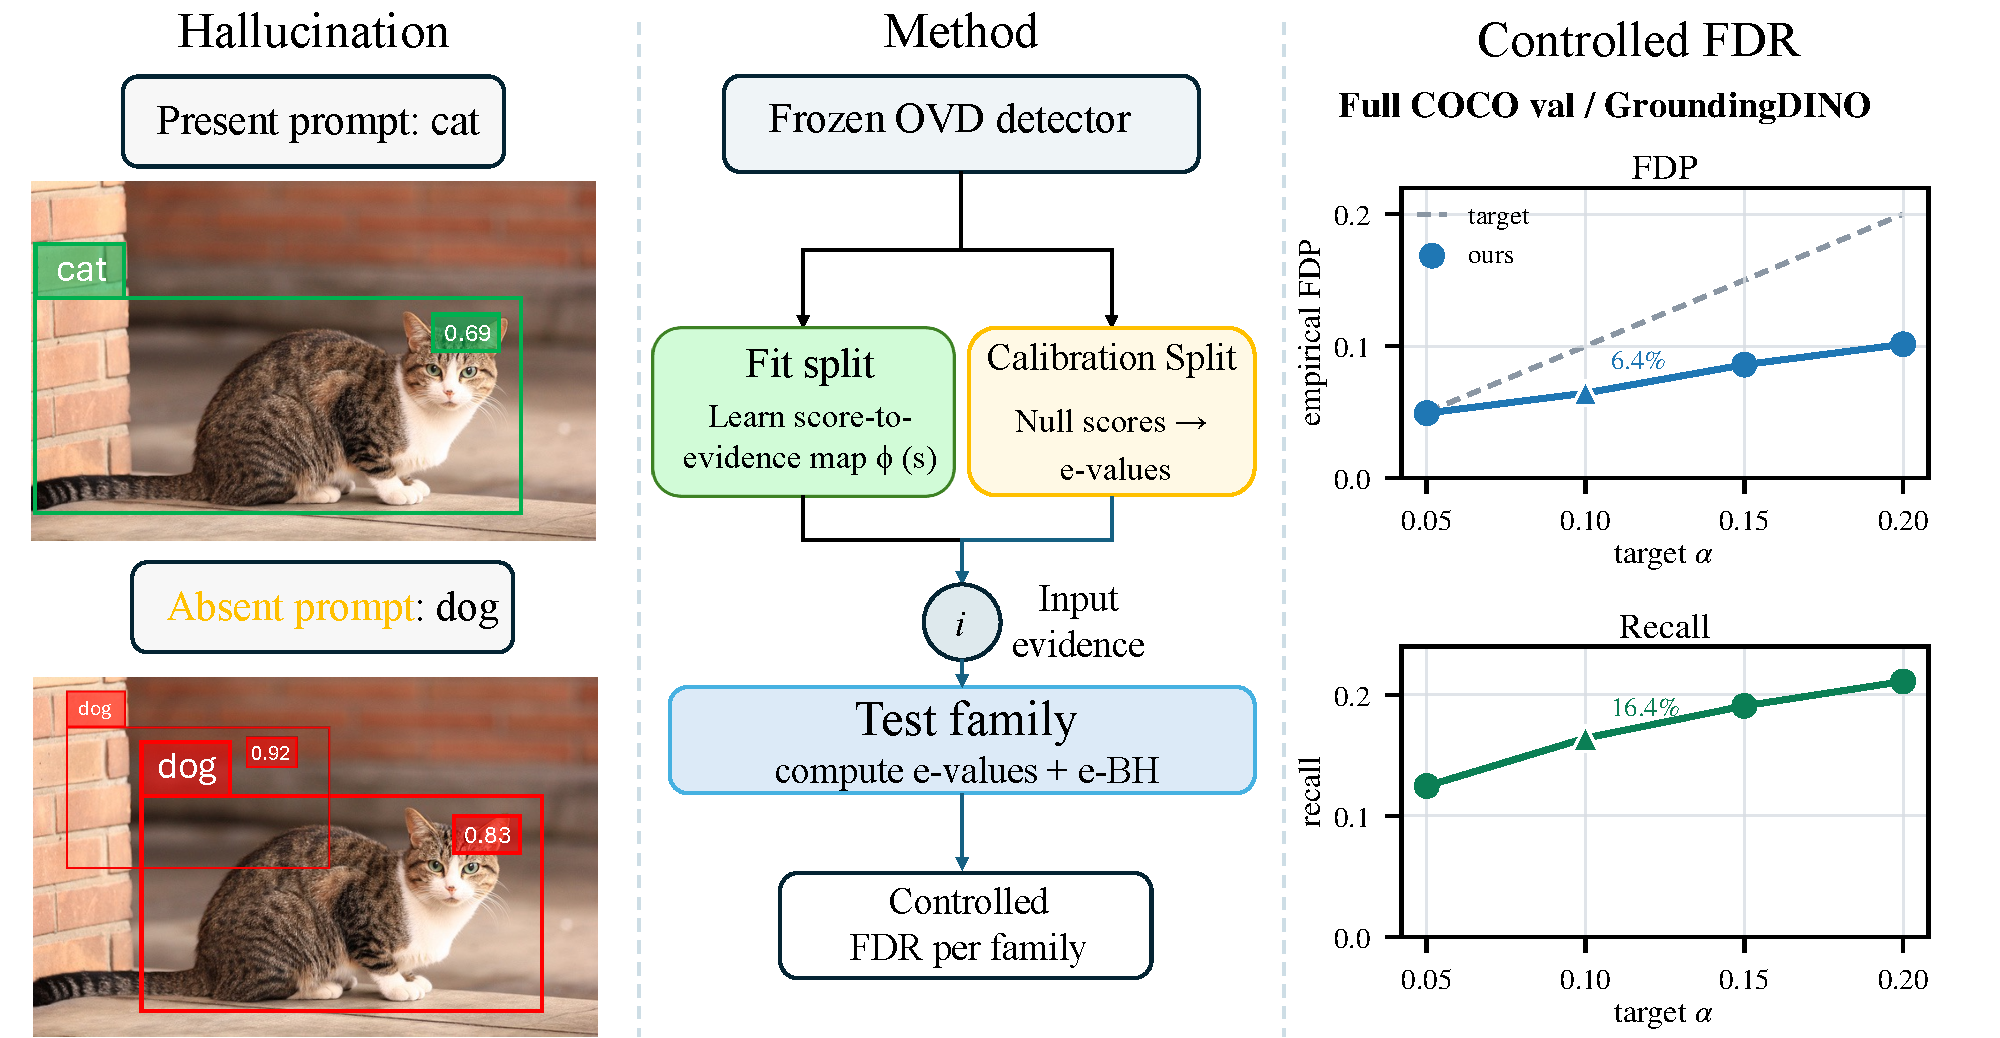
\includegraphics[width=\linewidth]{../outputs/paper_figures/fig_nips.pdf}
\vspace{-3mm}
\caption{Overview: absent-prompt boxes can score highly; our frozen-detector
wrapper converts scores to e-values and applies per-family e-BH to control FDR
with non-trivial recall.}
\label{fig:intro_teaser}
\vspace{-1mm}
\end{figure}

The method requires ``absent in the annotation'' to imply ``truly
absent''; this holds for exhaustive-per-class datasets (COCO, VOC), while
non-exhaustive annotations in LVIS~\cite{gupta2019lvis} and
Open Images~\cite{kuznetsova2020open} can sharply reduce power
unless contamination is bounded or the evaluation vocabulary is
curated
(Theorem~\ref{thm:true_label_fdr}; Section~\ref{sec:boundary}).
Our main experiments use category-name prompts and fixed template
banks for which absent/present status can be audited; fully
free-form language queries fall outside this setting and remain
future work.

We treat the frozen detector together with its score filter and NMS stack as a
deterministic candidate generator, and target finite-sample control of the
hallucination false discovery rate (FDR) on released detections within each
image-query family. The feasible-regime method has three steps. First, on a
held-out fit split, we learn a nonnegative score-to-evidence map $\phi$ by
matching candidates to ground truth and fitting a density-ratio style
estimator. Second, on a null-only calibration split, we turn each test
candidate score into a self-normalized conformal betting e-value. Its
validity follows from a one-line exchangeability argument
(Lemma~\ref{lem:exact_validity}) and does not require any concentration
inequality or clipping. Third, we apply e-BH~\cite{wang2022false} within
each image-query family, which yields valid FDR control under arbitrary
dependence among candidates in that family.

\paragraph{Contributions.}
We formulate image-query hallucination filtering as finite-sample
family-level FDR control under arbitrary within-family dependence
and derive the e-BH rejection condition
$T_r(K,C_m)=K C_m/[\alpha r(m{+}1){-}K]$ that characterizes its
power. Combined with the contamination analysis, this condition
leads to a deployment-level distinction between exhaustive
annotation, bounded contamination, and fixed-template calibration,
and suggests practical variants such as score filtering,
cluster-level aggregation, and template-specific calibration
(Section~\ref{sec:score_floor_exp},
Section~\ref{sec:nms_aware}, Appendix~\ref{app:freeform}).
Across COCO, VOC, Open
Images~\cite{kuznetsova2020open}, LVIS~\cite{gupta2019lvis}, and
four detectors (GroundingDINO, OWL-ViT, YOLO-World, RegionCLIP),
in the regimes where the null-pool assumption is auditable the
procedure controls per-family FDR; in regimes with non-exhaustive
annotation or score mixing, the observed failures match the
mechanisms analyzed by the rejection condition. A stratified concentration analysis yields
a non-vacuous pooled FDP bound on the majority of families
(Corollary~\ref{cor:stratified_pooled}).

\section{Related Work}
\label{sec:related}

Self-normalized conformal e-value validity and e-BH FDR control
are standard in the e-value literature. Our contribution is to
instantiate them for OVD hallucination filtering, to make the
resulting e-BH rejection condition explicit for detection families
(Theorem~\ref{thm:activation_frontier}), and to pair it with a
contamination analysis
(Theorems~\ref{thm:contamination}--\ref{thm:true_label_fdr})
relevant to non-exhaustive annotation. The condition is algebraic
but useful for diagnosing power loss in large, contaminated, or
score-mixed families. The main distinction from prior conformal
detection work is that we control released-box FDR for dependent
candidate boxes within an image-query family, rather than coverage
or recall-oriented risk.

\paragraph{OVD reliability.}
OVD detectors~\cite{gu2021open,zhong2022regionclip,li2022grounded,zhou2022detecting,du2022learning,kuo2022f,wu2023cora,yao2023detclipv2,zhang2023simple,wang2023open,li2024learning,zhao2024taming,kim2024region,cho2024language}
and open-set/open-world
variants~\cite{joseph2021towards,han2022expanding,sarkar2024open,yin2025rod,xi2025ow,zhang2025open,yang2025detecting}
target new-class coverage rather than reliability of released detections.
OVD-specific hallucinations and fine-grained failures are documented
in~\cite{ruis2026fantastic,bianchi2024devil};
BIRDet~\cite{zeng2024boosting} modifies detector representations,
whereas we wrap any frozen detector with a post-hoc finite-sample
guarantee.

\paragraph{Conformal multiple testing and e-values.}
Conformal prediction~\cite{angelopoulos2023conformal} and conformal
risk control~\cite{angelopoulos2022conformal} give distribution-free
coverage or risk bounds. In vision, SeqCRC~\cite{andeol:hal-05399935}
controls sequential detection risk and is recall-/loss-oriented, while
Conf-OT~\cite{silva2025conformal} adapts conformal prediction to
zero-shot image-label classification; other applications target
bounding-box uncertainty~\cite{timans2024adaptive} and
segmentation~\cite{mossina2025controlling}. These methods have
different targets than ours: none controls family-level FDR for
dependent candidate boxes released by an OVD pipeline.
Standard BH~\cite{benjamini1995controlling}/BY~\cite{benjamini2001control}
applied to conformal p-values requires
independence or PRDS and acts at the wrong granularity. We instead
build on e-values~\cite{vovk2021values}, e-BH~\cite{wang2022false},
and betting calibration~\cite{10.1093/jrsssb/qkad009}, but our
contribution is not their application:
Theorem~\ref{thm:activation_frontier} establishes a closed-form activation
frontier characterizing \emph{when} e-BH can reject in an image-query
family, and Corollary~\ref{cor:recall_ceiling} shows self-normalized
e-BH saturates it. These are not consequences of the e-BH guarantee,
which bounds FDR but says nothing about power.
Conformal e-values have appeared in novelty
detection~\cite{bashari2023derandomized}, but not OVD hallucination
filtering.
Other directions, including adaptive conformal
methods~\cite{gibbs2025conformal}, learned-score
FDR~\cite{marandon2022machine}, side-information
thresholding~\cite{lei2018adapt}, limited-FP prediction
sets~\cite{fisch2022conformal}, and defer-to-expert
systems~\cite{montreuil2024two}, do not address family-level FDR
under strong within-family dependence.

\paragraph{Label contamination and missing annotation.}
Missing-label detection work~\cite{xu2019missing,yang2020object}
motivates our contamination model (Section~\ref{sec:boundary}) but
addresses training, not post-hoc control. Contamination and group-shift
results~\cite{bates2023testing,barber2023conformal} are complementary
to our $1/\eta$ saturation ceiling and graceful-degradation analysis:
they characterize how validity degrades under an impure null pool,
while the rejection condition of Theorem~\ref{thm:activation_frontier}
indicates when that degradation becomes a zero-power phase transition
for OVD families.

\section{Problem Setup}
\label{sec:setup}

Let $x$ denote an image and let $q$ denote a text prompt, such as a category name or a free-form phrase. Fix a frozen open-vocabulary detector together with its score thresholding and non-maximum suppression pipeline, and treat the whole stack as a deterministic candidate generator
\begin{equation}
G_f(x, q) = \{(b_k, s_k)\}_{k=1}^{K(x,q)},
\end{equation}
where the subscript $f=(x,q)$ indexes the image-query \emph{family}, $b_k$ is a candidate box, $s_k \in \mathbb{R}$ is its detector score, and $K(x,q)$ is the data-dependent family size after post-processing.

We observe a calibration dataset
\begin{equation}
\mathcal{D}_{\mathrm{cal}} = \{(x_i, q_i, B_i^\star)\}_{i=1}^n,
\end{equation}
where $B_i^\star$ is the set of ground-truth boxes matching prompt $q_i$ in image $x_i$. The statistical assumption is that, under the null hypothesis for a given test candidate, its score is exchangeable with the null scores from the calibration split, conditional on the fit split. This is a within-null-pool assumption; it does \emph{not} require exchangeability across families or between true positives and nulls. Within a family we allow arbitrary dependence among candidate boxes, which matters in this setting because proposal sharing and NMS induce strong and unmodelable dependence. Pooling null scores across families is justified when they share a common null score distribution; our LOO diagnostic (mean $=1.000$ on all configurations) is consistent with this assumption. Appendix~\ref{app:proofs} gives a formal approximate-exchangeability bound under mild groupwise shift.

For a candidate $b_k$ from a test family $(x,q)$, define the null hypothesis
\begin{equation}
H_k^0:\quad b_k \text{ is unmatched under greedy IoU matching at threshold } \tau,
\end{equation}
where greedy matching assigns each ground-truth box to at most one detection
(highest IoU first; see Appendix~\ref{app:benchmark} for details).
A true null thus corresponds to a hallucinated detection. We use $\tau=0.5$ throughout (the standard COCO criterion) and verify robustness to $\tau\in\{0.3,0.7\}$ in Appendix~\ref{app:iou_sensitivity}. When $B^\star=\varnothing$, every candidate in the family is null.

\paragraph{Query-vocabulary annotation.}
The null pool requires ``absent in the annotation'' to imply ``truly
absent'' only for the \emph{queried categories}. This is strictly
weaker than full per-class exhaustive annotation and applies
whenever the deployment vocabulary is known at calibration time.

The goal is a selection rule $\mathcal{S}$ that releases a subset of candidates while controlling
\begin{equation}
\FDR(\mathcal{S}) = \E\left[\frac{|\{k : \mathcal{S}_k=1,\ H_k^0\ \text{true}\}|}{|\{k : \mathcal{S}_k=1\}| \vee 1}\right]
\le \alpha
\end{equation}
for a user-specified level $\alpha \in (0,1)$, in finite samples, without any within-family independence assumption.

Family-level FDR is the primary target because each image-query
pair is a natural invocation of the OVD system; this also prevents
a few large families from dominating the risk. Pooled FDP, the
ratio of false discoveries to total releases across families, is
reported as an empirical global-precision diagnostic, with a
non-vacuous concentration certificate on the $K\!\le\!5$ stratum
(Corollary~\ref{cor:stratified_pooled}). The exchangeability
assumption is a calibration assumption on the null pool, not an
independence assumption among detections; it may fail under
prompt- or dataset-level shifts, and our LOO diagnostic detects
only gross violations.

\section{Method}
\label{sec:method}

The procedure has three components: labeling TP and null scores on
a fit split, calibrating self-normalized e-values on a null-only
split, and applying e-BH within each image-query family on the test
split. The detector is not modified and no within-family
independence is assumed.

\subsection{Three-Split Protocol}

The procedure uses three disjoint family-level splits. On the
\emph{fit} split (60\% of families), we apply greedy IoU matching
(\S\ref{sec:setup}) to label candidates as TP ($y_{i,k}\!=\!1$) or
null, and learn a score-to-evidence map $\phi(s)$. On the
\emph{calibration} split (20\%), we retain null candidates only;
these are used solely to self-normalize test e-values and never to
fit $\phi$. On the \emph{test} split (20\%), we compute one e-value
per candidate and apply e-BH within each family. Splits are taken
by family identifier so intra-family dependence is preserved.

The fit split yields a nonnegative score transform
$\phi : \mathbb{R} \to \mathbb{R}_{\ge 0}$, interpretable as a
density-ratio estimate $\phi(s)\approx\hat{p}_1(s)/\hat{p}_0(s)$.
Our default is an unsmoothed 80-bin histogram
(KDE/logistic/isotonic ablations in
Appendix~\ref{app:additional}); validity requires only that $\phi$
be deterministic given the fit split, so estimator quality affects
power, not validity.

\subsection{Self-Normalized Conformal Betting e-Values}

The self-normalized e-value below builds on conformal e-value
constructions~\cite{vovk2021values,wang2022false}; the
detection-specific power theory
(Theorem~\ref{thm:activation_frontier}) that follows is new.

Fix a test candidate score $S$ whose null hypothesis is true, and let
\begin{equation}
S_1^{\mathrm{cal}}, \dots, S_m^{\mathrm{cal}}
\end{equation}
be the null scores from the calibration split. Conditional on the fit split, assume the null scores are exchangeable:
\begin{equation}
(S, S_1^{\mathrm{cal}}, \dots, S_m^{\mathrm{cal}})
\ \text{exchangeable under } H^0.
\end{equation}
Define the self-normalized e-value
\begin{equation}
e(S)
=
\frac{(m+1)\phi(S)}
{\phi(S) + \sum_{j=1}^m \phi(S_j^{\mathrm{cal}})}.
\label{eq:self_normalized_evalue}
\end{equation}

Relative to mean-centering alternatives, this construction absorbs calibration randomness into the denominator itself and therefore yields an exact finite-sample validity statement rather than a high-probability approximation.
It is also closely aligned with the betting/e-value viewpoint in modern
sequential inference \cite{vovk2021values,10.1093/jrsssb/qkad009}.

\begin{lemma}[Exact validity of the self-normalized e-value]
\label{lem:exact_validity}
Condition on the fit split and suppose $(S, S_1^{\mathrm{cal}}, \dots, S_m^{\mathrm{cal}})$ is exchangeable under $H^0$. Let $\phi$ be any deterministic nonnegative function of the score. Then the e-value in \eqref{eq:self_normalized_evalue} is valid:
\begin{equation}
\E_{H^0}[e(S)] \le 1.
\end{equation}
In fact, if $\phi(S) + \sum_{j=1}^m \phi(S_j^{\mathrm{cal}}) > 0$ a.s., equality holds ($\E_{H^0}[e(S)] = 1$).
\end{lemma}

\emph{Proof sketch.} By exchangeability, $\phi(S_j)/T$ have equal
expectation for $j=0,\ldots,m$ where $T=\sum_{j=0}^m \phi(S_j)$;
summing gives $\E[\phi(S_0)/T]=1/(m{+}1)$. Full proof in
Appendix~\ref{app:proofs}. Validity is unconditional on $\phi$;
the role of $\phi$ is purely to shape power, enabling the
detection-specific power theory that follows.

\subsection{Per-Family e-BH for Arbitrary Within-Family Dependence}

Consider a test family with candidate e-values $e_1,\dots,e_K$. We apply e-BH at level $\alpha$ within that family. Let $e_{(1)} \ge \dots \ge e_{(K)}$ denote the sorted e-values and define
\begin{equation}
\hat{k} = \max\left\{k \in \{1,\dots,K\} : e_{(k)} \ge \frac{K}{\alpha k}\right\},
\end{equation}
with the convention $\hat{k}=0$ if the set is empty. The rejection set is then
\begin{equation}
\R = \{j : e_j \ge e_{(\hat{k})}\}.
\end{equation}

We work with e-values rather than p-values to sidestep the
dependence issue. Standard BH~\cite{benjamini1995controlling}
requires independence or positive dependence
assumptions~\cite{benjamini2001control} that are difficult to
justify after proposal generation and NMS, whereas
e-BH~\cite{wang2022false} accommodates arbitrary dependence once
the input e-values are valid.

\begin{proposition}[Per-family FDR control]
\label{prop:family_fdr}
Suppose every null candidate in a test family is assigned a valid e-value by \eqref{eq:self_normalized_evalue}. Then e-BH at level $\alpha$ satisfies
\begin{equation}
\E\left[\frac{|\R \cap \Hnull|}{|\R| \vee 1}\right] \le \alpha
\end{equation}
for that family, regardless of the dependence structure among the candidates in the family.
\end{proposition}

Averaging over the test-family distribution immediately gives a marginal
family-averaged FDR guarantee as well.
Appendix~\ref{app:proofs} also gives a hierarchical extension: construct
family-level e-values from an independent split, run e-BH across families, and
then run within-family e-BH on the selected families. This controls family
selection FDR together with selected-family mean FDP.

\subsection{Activation Frontier for Image-Query Families}

Lemma~\ref{lem:exact_validity} and Proposition~\ref{prop:family_fdr}
establish validity. Power, i.e., whether e-BH actually rejects any
candidates in a family, requires a separate characterization.

Theorem~\ref{thm:activation_frontier} below gives the necessary and
sufficient condition in one line: \emph{the $r$-th rejection in a family of size $K$
is possible iff the $r$-th largest evidence exceeds
$K C_m / [\alpha r(m{+}1){-}K]$}. Several consequences used below
follow from this condition.

\begin{theorem}[Family activation frontier]
\label{thm:activation_frontier}
Consider a test family of size $K$ with candidate $\phi$-values sorted as
$\phi_{(1)} \ge \phi_{(2)} \ge \cdots \ge \phi_{(K)}$.
Let $C_m = \sum_{j=1}^m \phi(S_j^{\mathrm{cal}})$ denote the calibration
pool aggregate. Then e-BH at level $\alpha$ rejects at least $r$ candidates
in this family if and only if
\begin{equation}
\phi_{(r)} \;\ge\; T_r(C_m)
\;:=\; \frac{K \, C_m}{\alpha\, r\, (m+1) - K},
\label{eq:activation_threshold}
\end{equation}
provided $\alpha\, r\, (m+1) > K$. If $\alpha\, r\, (m+1) \le K$, the
$r$-th rejection is structurally impossible regardless of the evidence.
\end{theorem}

The proof follows by substituting the e-value definition into the e-BH
criterion and rearranging; see Appendix~\ref{app:proofs}.

\begin{corollary}[Frontier saturation]
\label{cor:recall_ceiling}
Call a true positive \emph{frontier-reachable} in family~$g$ if it is
among the top-$R_g$ candidates by~$\phi$, where
$R_g=\max\{r:\phi_{(r,g)}\ge T_r(C_m)\}$ is the maximum number of
rejections permitted by Theorem~\ref{thm:activation_frontier}. Then
self-normalized e-BH rejects a candidate if and only if it is
frontier-reachable.
\end{corollary}

The identity is algebraic. Since
$e(S)=(m\!+\!1)\phi(S)/[\phi(S)+C_m]$ is strictly increasing
in~$\phi$, sorting by e-value coincides with sorting by~$\phi$, and
the e-BH selection count equals~$R_g$
(Appendix~\ref{app:proofs}). Consequently, the gap between observed
recall and $100\%$ reflects TPs whose density ratios fall below the
family activation threshold, which is a property of the detector's
score geometry rather than of the procedure. Improving recall therefore requires either improving $\phi$
(sharper estimator or stronger detector scores) or reducing the
effective family size~$K$ (Remark~\ref{rem:score_floor}), not the
testing procedure.
Theorem~\ref{thm:activation_frontier} and
Corollary~\ref{cor:recall_ceiling} together explain binary
e-values' powerlessness, high-$K$ families' stricter thresholds, and
contamination's effect on~$C_m$
(Section~\ref{sec:boundary}).

\begin{remark}[Frontier descent via deterministic pre-screening]
\label{rem:score_floor}
Theorem~\ref{thm:activation_frontier} shows that $T_r$ grows with
family size~$K$. A deterministic score floor $s_{\mathrm{floor}}$,
fixed a priori or chosen on the fit split, removes candidates with
score $<s_{\mathrm{floor}}$ from each test family. The result is an
effective size $K_{\mathrm{eff}}\le K$ and strictly lower activation
thresholds. Validity is preserved: each
surviving candidate's e-value~\eqref{eq:self_normalized_evalue} depends
only on the calibration pool (unchanged) and its own~$\phi$, so
Lemma~\ref{lem:exact_validity} applies to any deterministic subset.
The recall trade-off is transparent: the floor discards TPs with
score below $s_{\mathrm{floor}}$, but the surviving TPs face a lower
activation barrier. The net effect is a substantial recall gain
whenever the detector assigns sufficiently distinct scores to TPs
and nulls (Section~\ref{sec:score_floor_exp}).
\end{remark}

\paragraph{Implementation details.}
We split by family identifier (not by candidate) so that intra-family
dependence is preserved. Only null candidates enter the calibration
pool~\eqref{eq:self_normalized_evalue}, keeping exchangeability exact.
The detector is frozen; we learn only a one-dimensional score map
(unsmoothed histogram by default).

\subsection{Cluster-level e-values under NMS-induced dependence}
\label{sec:nms_aware}

Detectors without internal NMS produce $5$--$20$ overlapping candidates
per object, diluting per-candidate budget. We partition candidates by
the undirected NMS graph ($\IoU\ge\tau$, connected components) and
assign one e-value per cluster $C$:
\begin{equation}
\label{eq:cluster_evalues}
E_{\mathrm{unif}}(C) = \tfrac{1}{|C|}\!\sum_{i\in C}\! E_i,
\qquad
E_{\mathrm{cal}}(C) = \tfrac{(n+1)\,R(C)}{R(C)+\sum_{j=1}^{n} R(C^{\mathrm{cal}}_j)},
\;\; R(C)=\max_{i\in C}\phi(s_i),
\end{equation}
where $E_i$ is~\eqref{eq:self_normalized_evalue} and
$\{C^{\mathrm{cal}}_j\}$ is a null-only pool of calibration clusters
exchangeable with test clusters under $H_0$.

\begin{proposition}[Cluster-level validity]
\label{prop:calibrated_cluster}
$\mathbb{E}_{H_0}[E_{\mathrm{unif}}(C)]\le1$ (closure under predictable
convex combinations) and
$\mathbb{E}_{H_0}[E_{\mathrm{cal}}(C)]\le1$ (self-normalized
construction of~\citet{vovk2021values} at cluster granularity). Per-family
e-BH on either e-value controls TP-cluster FDR at~$\alpha$ (Appendix~\ref{app:nms_aware_proofs}).
\end{proposition}

Proposition~\ref{prop:calibrated_cluster} establishes cluster-level
validity. Empirically, predictable uniform aggregation is conservative,
whereas calibrated score-adaptive weighting improves object-level
power: uniform averaging dilutes a cluster with one strong and ten weak
members, while calibrating $R_{\max}$ against null clusters does not. When $\tau$ is so high that every cluster is a
singleton, $E_{\mathrm{cal}}$ reduces exactly
to~\eqref{eq:self_normalized_evalue} and gracefully recovers the
candidate baseline.

\section{Experiments}
\label{sec:experiments}

We evaluate whether the proposed wrapper controls per-family FDR
on frozen OVD detectors while retaining non-trivial recall.

\subsection{Setup}

We evaluate on COCO val 2017~\cite{lin2014microsoft} (4{,}952 images) and
Pascal VOC 2012 val~\cite{everingham2010pascal}, both exhaustively annotated.
Three detectors span distinct architectures:
GroundingDINO~\cite{liu2024grounding},
OWL-ViT~\cite{minderer2022simple}, and
YOLO-World~\cite{cheng2024yolo}. Each image is paired with one present
and two absent prompts ($3{,}000$ families per 1k-image configuration),
split 60/20/20 (fit/cal/test) by family. The score map $\phi$ is an
unsmoothed 80-bin histogram. Numbers are means $\pm$ s.d.\ over 20 random
splits unless noted. Appendix~\ref{app:benchmark} specifies the prompt
set, template bank, detector score thresholds and NMS settings, random
seeds ($0$--$19$), split construction, and histogram binning used in
all experiments.

\subsection{Main Result: Per-Family FDR Control on COCO and VOC}

Table~\ref{tab:main_fullscale} reports the core evaluation on full
COCO val with GroundingDINO. The primary metric is per-family FDR
(Proposition~\ref{prop:family_fdr}); pooled FDP is diagnostic. At
$\alpha\!=\!0.10$, per-family mean FDP is well below nominal across
all six configurations (Table~\ref{tab:coverage_1k}; max $1.69\%$),
pooled FDP is $6.44\%$ (19/20 pass), recall is $16.4\%$, and released
detections have $93.6\%$ empirical pooled precision vs.\ $72.9\%$
for $p$-value BH; LOO mean is $1.000$. Cross-detector 1k-subset
coverage in App.~\ref{app:coverage_1k}.

\begin{table}[t]
\centering
\small
\begin{tabular*}{\linewidth}{@{\extracolsep{\fill}}c|cccc|cc@{}}
\toprule
& \multicolumn{4}{c}{Betting e-BH (ours)} & \multicolumn{2}{c}{Baselines} \\
\cmidrule(lr){2-5}\cmidrule(lr){6-7}
$\alpha$ & Rej.\ & Per-family FDP & Pooled FDP & Recall & Pooled FDP (p-BH) & Recall (binary) \\
\midrule
0.05 & $459.6$ & $\mathbf{0.43\%}$ & $4.9\%$ & $12.5\%$ & $17.9\%$ & $0.16\%$ \\
0.10 & $615.1$ & $\mathbf{0.78\%}$ & $6.4\%$ & $16.4\%$ & $27.1\%$ & $0.18\%$ \\
0.15 & $731.4$ & $\mathbf{1.10\%}$ & $8.6\%$ & $19.1\%$ & $35.0\%$ & $0.19\%$ \\
0.20 & $823.0$ & $\mathbf{1.45\%}$ & $10.1\%$ & $21.1\%$ & $42.3\%$ & $0.83\%$ \\
\bottomrule
\end{tabular*}
\caption{Full-scale COCO val (4{,}952 images) with GroundingDINO, 20 random
splits. Per-family FDP (Proposition~\ref{prop:family_fdr}) $\ll\alpha$ at
every level; pooled FDP is diagnostic at full-family scale;
a stratified empirical Bernstein bound
(Corollary~\ref{cor:stratified_pooled}) is non-vacuous on the
$K\!\le\!5$ stratum (57\% of families). p-value BH violates pooled target;
binary e-BH has negligible recall. Pass rate at $\alpha=0.10$: 19/20.}
\label{tab:main_fullscale}
\end{table}

Figure~\ref{fig:alpha_sweep} shows full risk curves across
$\alpha\in\{0.05,0.10,0.15,0.20\}$: empirical FDP stays strictly below
the nominal level and recall grows monotonically with $\alpha$.
OWL-ViT's lower FDP reflects its smaller families ($K\!\approx\!2.5$
vs.\ $10$).

\begin{figure}[t]
\centering
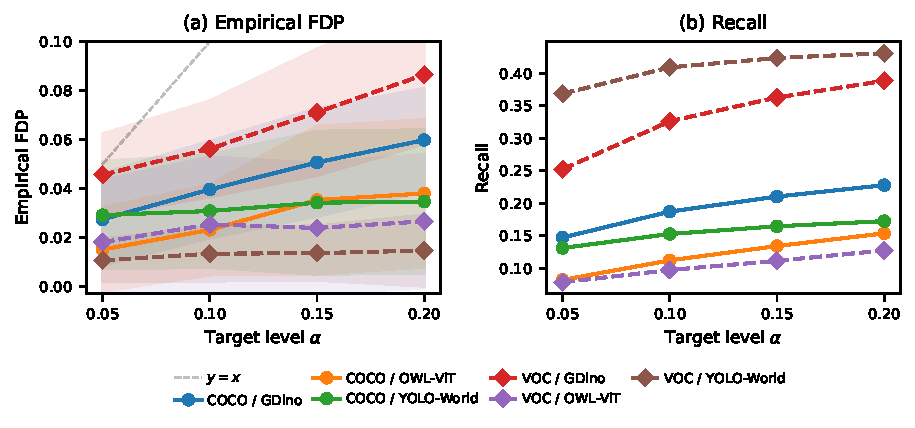
\includegraphics[width=\linewidth]{../outputs/paper_figures/fig1_alpha_sweep.pdf}
\caption{Risk curves ($\alpha\!\in\!\{0.05,\ldots,0.20\}$, six
configs, $1{,}000$-image subsets, 20 splits; full-scale in
Table~\ref{tab:main_fullscale}).
(a)~FDP stays below $y\!=\!x$. (b)~Recall grows with $\alpha$.
Solid: COCO; dashed: VOC.}
\label{fig:alpha_sweep}
\end{figure}

On the 1{,}000-image subsets (Figure~\ref{fig:alpha_sweep}), all
six configurations attain 20/20 pooled-FDP pass at
$\alpha\!\ge\!0.10$ (Appendix~\ref{app:20seed}); the full-scale
COCO/GDino row in Table~\ref{tab:main_fullscale} is 19/20 at
$\alpha\!=\!0.10$. COCO-train confirms with exact LOO validity
(Appendix~\ref{app:coco_train}). By
Corollary~\ref{cor:recall_ceiling}, the residual recall gap is a
detector-side limitation; score-floor pre-screening lifts recall to
$33.3\%$/$49.0\%$ on COCO/VOC
(Section~\ref{sec:score_floor_exp}). Pooled FDP admits a finite-sample concentration bound
(Proposition~\ref{prop:pooled_concentration}); an empirical Bernstein
refinement on the $K\!\le\!5$ stratum yields a non-vacuous certificate
$\varepsilon\!=\!0.074$ (Appendix~\ref{app:pooled_fdp}).

\subsection{Comparison with Thresholding and $p$-Value Procedures}

We compare against a broad set of thresholding, $p$-value,
risk-control, and adaptive multiple-testing baselines using the same
candidate pools and calibration splits. Table~\ref{tab:baselines}
summarizes the comparison.

For $p$-value baselines, we compute conformal $p$-values
$p(s)\!=\!(1+|\{j:S_j^{\mathrm{cal}}\!\ge\!s\}|)/(m{+}1)$ and apply
BH/BY~\cite{benjamini1995controlling,benjamini2001control} per family.
\emph{Calibration-tuned thresholding} picks the lowest threshold with
calibration FDP $\le\alpha$; it reaches $31.6\%$ recall but fails 13/20
splits, since the cal-to-test concentration correction
($\varepsilon\!\approx\!0.12$) consumes the budget. $p$-BH and BY
violate the pooled target ($27.7\%/11.3\%$); binary e-BH is valid but
powerless. VOC/GDino shows the same pattern; results are robust to
estimator and cal pool size (App.~\ref{app:additional},~\ref{app:cal_size}).

\begin{table}[t]
\centering
\small
\begin{tabular*}{\linewidth}{@{\extracolsep{\fill}}lccccc@{}}
\toprule
Method & Rej.\ & Pooled FDP & Per-family FDP & Recall & Pass? \\
\midrule
Raw detector (no filter) & $6164$ & $88.7\%$ & --- & $100\%^{\dagger}$ & $\times$ \\
Cal.\ threshold~\cite{angelopoulos2022conformal,fisch2022conformal} & $240$ & $10.0\%$ & $7.09\%$ & $31.6\%$ & $\times$ \\
p-value BH~\cite{bates2023testing,benjamini1995controlling} & $383$ & $27.7\%$ & $5.54\%$ & ---$^{*}$ & $\times$ \\
p-value BY~\cite{bates2023testing,benjamini2001control} & $212$ & $11.3\%$ & $3.29\%$ & $27.7\%$ & $\triangle$ \\
Top-$k$ per family (cal-tuned)~[E2] & $537$ & $67.4\%$ & $67.4\%$ & $25.5\%$ & $\times$ \\
CRC (mean-family risk)~\cite{angelopoulos2024conformal} & $521$ & $33.9\%$ & $9.73\%$ & $49.1\%$ & $\times$ \\
Storey-BH~\cite{storey2002direct} & $514$ & $39.7\%$ & $20.3\%$ & $41.1\%$ & $\times\times$ \\
BKY two-stage~\cite{benjamini2006adaptive} & $414$ & $30.2\%$ & $18.2\%$ & $39.0\%$ & $\times\times$ \\
IHW-lite (cov.\ $K$)~\cite{ignatiadis2016data} & $209$ & $8.07\%$ & $7.90\%$ & $27.5\%$ & $\triangle$ \\
Binary e-BH~\cite{vovk2021values,wang2022false} & $2$ & $1.6\%$ & $0.08\%$ & $0.2\%$ & \checkmark \\
\textbf{Betting e-BH (ours)} & $\mathbf{134}$ & $\mathbf{3.96\%}$ & $\mathbf{0.65\%}$ & $\mathbf{18.7\%}$ & \checkmark \\
\bottomrule
\end{tabular*}
\vspace{1pt}

\caption{Baseline comparison, COCO-1k/GDino, $\alpha=0.10$, 20 seeds.
\checkmark/$\triangle$/$\times$/$\times\times$ = all pass / partial / pooled fails / pooled and per-family both fail.
$^{*}$pooled FDP violated; $^{\dagger}$candidate-level recall is trivially $100\%$
when all candidates are released.
[E2]: top-$k$ baseline picks largest $k$ with cal mean family-FDP~$\le\!\alpha$
(Appendix~\ref{app:strong_baselines}).
IHW-lite uses family size $K$ (binned) as the covariate; see
Appendix~\ref{app:strong_baselines} for the full per-config breakdown.}
\label{tab:baselines}
\end{table}

\subsection{Score-Floor Pre-Screening: Activation-Frontier Descent}
\label{sec:score_floor_exp}

A deterministic pre-screen shrinks $K_{\mathrm{eff}}$ and hence $T_r$
(Remark~\ref{rem:score_floor}). The fit-split-selected \emph{adaptive}
floor ($s_{\mathrm{floor}}^{\star}\!\approx\!0.05$--$0.10$, no test
labels) is the pooled-safe default; the fixed $0.40$ floor is a
recall-oriented operating point that consumes pooled-FDP slack
(Table~\ref{tab:score_floor}). Per-family FDR holds at both; the
choice maps to deployment Mode~A vs B/C
(App.~\ref{app:score_floor_cross}).

\begin{table}[t]
\centering
\small
\begin{tabular*}{\linewidth}{@{\extracolsep{\fill}}llcccccc@{}}
\toprule
Config & $s_{\mathrm{floor}}$ & Rej.\ & Per-fam.\ FDP & Pooled FDP & Recall & Pass & Gain \\
\midrule
\multirow{2}{*}{COCO/GDino}
& $0.05$ (\textbf{adaptive})& $134$ & $0.65\%$ & $4.0\%$  & $18.7\%$ & $1.00$ & --- \\
& $0.40$ (fixed)            & $261$ & $2.59\%$ & $11.5\%$ & $33.3\%$ & $0.30$ & $1.78\times$ \\
\midrule
\multirow{2}{*}{VOC/GDino}
& $0.05$ (\textbf{adaptive})& $196$ & $1.69\%$ & $5.6\%$  & $32.6\%$ & $1.00$ & --- \\
& $0.40$ (fixed)            & $317$ & $4.42\%$ & $12.0\%$ & $49.0\%$ & $0.40$ & $1.50\times$ \\
\bottomrule
\end{tabular*}
\caption{Score-floor pre-screening at $\alpha=0.10$ (1k images, GDino,
20 seeds). Per-family FDP $\ll\alpha$ at every floor (Proposition~\ref{prop:family_fdr}
holds finite-sample). Pooled FDP and pass rate (fraction of seeds with
pooled FDP $\le\alpha$) reveal the deployment trade: the
fit-split-selected \emph{adaptive} floor ($\approx\!0.05$, chosen on fit nulls only)
is the principled default; the aggressive fixed $0.40$ trades $1.5$--$1.8\times$
recall for pooled-FDP slack at $\alpha\!=\!0.10$.}
\label{tab:score_floor}
\end{table}

\paragraph{Object-level recall via cluster e-BH.}
The calibrated cluster e-value $E_{\mathrm{cal}}$
(Section~\ref{sec:nms_aware}, $\tau\!=\!0.5$, $R_{\max}$) lifts recall
$1.4$--$1.8\times$ at matched FDP: at $\alpha\!=\!0.10$,
$18.7\%\!\to\!32.1\%$ COCO/GDino, $32.6\%\!\to\!54.3\%$ VOC/GDino,
$3.7\%\!\to\!21.6\%$ COCO/RegionCLIP ($5.8\times$, no internal NMS;
App.~\ref{app:obj_vs_cand}). Stratified diagnostics by score
quantile, object size, and category
(App.~\ref{app:conditional_validity}) show no systematic calibration
failure: rejections concentrate in the top score quintile, object-size
pooled FDP is at or near $\alpha$ on COCO/GDino across sizes, and
per-family FDR holds within every category; per-category pooled FDP
is a stress diagnostic only.

\section{A Three-Regime Deployment Map}
\label{sec:boundary}

The rejection condition (Theorem~\ref{thm:activation_frontier}) and
contamination saturation (Theorem~\ref{thm:contamination}) define
three regimes with distinct failure modes
(Figure~\ref{fig:intro_teaser}, middle panel).

\subsection{Regime I --- Exhaustive Annotation (Feasible)}

On COCO/VOC, $\alpha$-validity holds and power is governed by $T_r$
(baseline recall $16$--$41\%$, Table~\ref{tab:main_fullscale};
Cor.~\ref{cor:recall_ceiling}); frontier-descent fixes lift recall to
$33\%/49\%$ (score floor) and $1.4$--$5.8\times$ (cluster).

\subsection{Regime II --- Bounded Contamination (Boundary)}

Non-exhaustive annotation contaminates the null pool with true positives.

\begin{theorem}[Contamination saturation of the density ratio]
\label{thm:contamination}
Let $r(s)=p_1(s)/p_0(s)$ be the clean density ratio. If an $\eta$ fraction
of the observed null pool is unlabeled positives, so
$q_0=(1-\eta)p_0+\eta p_1$, then
\begin{equation}
\phi_\eta(s)
= \frac{p_1(s)}{q_0(s)}
= \frac{r(s)}{1-\eta+\eta\,r(s)}
\label{eq:contaminated_phi}
\end{equation}
satisfies $\phi_\eta\le1/\eta$ and compresses high-evidence regions;
$\eta$ is identified from $r_{\max},M\!=\!\sup\phi_\eta$ via
$\eta=(r_{\max}-M)/[M(r_{\max}-1)]$.
\end{theorem}

\begin{theorem}[True-label FDR under contamination]
\label{thm:true_label_fdr}
For $q_0=(1-\eta)p_0+\eta p_1$, any $q_0$-valid e-value satisfies
$\mathbb{E}_{p_0}[E]\le1/(1-\eta)$; e-BH at level $\alpha$ thus
controls true-label FDR at $\alpha/(1-\eta)$, restored to $\alpha$
under level $\alpha(1-\bar\eta)$ when $\eta\le\bar\eta$, with a
zero-rejection phase transition when $1/\eta<T_1(C_m)$
(Cor.~\ref{cor:phase_transition}).
\end{theorem}

\paragraph{Controlled contamination.}
Hiding $\eta_{\mathrm{fam}}\!\in\!\{0,\ldots,0.50\}$ on COCO/VOC
validates Theorem~\ref{thm:contamination}
(Fig.~\ref{fig:contamination_sweep}, Table~\ref{tab:contamination_detail}):
$\phi_{\max}$ tracks $1/\eta$, true FDP stays controlled, recall
collapses. Three LVIS repairs fail (App.~\ref{app:repair});
$\hat\eta$-correction ($38$ rejections, $0.99\%$ FDP) and vocabulary
curation (App.~\ref{app:a1_honest}, $11$--$21\%$ recall) address
opposite ends of the chain.

\subsection{Regime III --- Fixed-Template Deployment (Score-Mixing Compression)}

Fixed template banks create a different bottleneck:
\emph{score-mixing compression} (Proposition~\ref{prop:mixing_compression})
drives $\sup\phi_{\mathrm{pool}}\!\approx\!14\!\ll\!T_1\!\approx\!283$
under pooling; per-template fitting recovers $98.6$ rejections at
$3.9\%$ FDP (App.~\ref{app:freeform}). Template count is bounded by
calibration ($T_{\mathrm{crit}}\!\propto\!N_{\mathrm{img}}/K_{\min}^{\mathrm{cal}}$).

\section{Discussion and Conclusion}
\label{sec:discussion}

We presented a post-hoc reliability wrapper for frozen
open-vocabulary detectors that controls family-level hallucination
FDR for auditable category-name or fixed-template prompts. The
statistical mechanism is simple: self-normalized conformal betting
e-values give finite-sample validity under null-score
exchangeability, and e-BH gives dependence-robust FDR control within
each image-query family. The diagnostic contribution is the
activation frontier $T_r(K,C_m)$, which separates validity from
power and explains three otherwise confusing phenomena: binary
e-values can be valid but powerless, large candidate families
impose high evidence thresholds, and contaminated null pools create
a zero-power phase transition. This view yields three practical
variants---adaptive score floors, cluster aggregation, and
template-specific calibration---each addressing one bottleneck.
Deployment distinguishes three modes: per-family FDR control,
empirical pooled-FDP/LOO diagnostics, and Bernstein-certified
pooled-FDP bounds on the $K\!\le\!5$ stratum. The method is a
release filter, not a detector improvement; validity depends on
auditable absence labels and deployment-specific contamination bounds.

\bibliographystyle{unsrtnat}
\bibliography{refs}

\newpage
\appendix
% Use numeric appendix numbering (we now have >26 sections)
\renewcommand{\thesection}{\Roman{section}}

\section{Repair Attempts on LVIS}
\label{app:repair}

We tested three targeted repairs on LVIS:
(i)~Mondrian splitting by absent/present status to isolate cleaner null strata;
(ii)~a minimum family-size filter ($k_{\min}$) to remove high-variance small families;
(iii)~a null-floor regularizer on $\phi$ to cap density-ratio blowup.
None of the three restored FDR control. With $\phi_{\max}\approx30$,
the signal content of the null pool is already too degraded for
e-BH to distinguish hallucinations from genuine detections at a
controlled rate, and none of the three patches closes the
annotation gap.

These results suggest that the limiting factor on LVIS is the
quality of the null pool rather than the particular post-hoc tuning
choice. They are consistent with the contamination mechanism
analyzed in Theorem~\ref{thm:contamination} and indicate that the
oracle-null assumption is not satisfied on LVIS at the scale we
evaluated.

\section{Honest Restricted Evaluation on LVIS and OpenImages}
\label{app:a1_honest}

In-place statistical repairs (Appendix~\ref{app:repair}) cannot restore
validity on LVIS/OI because the annotation signal is the missing
component. A complementary strategy is to \emph{curate} the evaluation
pool so that the oracle-null assumption holds: remove families whose
absence cannot be certified, then run the unmodified pipeline. The contamination boundary is addressed from two sides. In-place
$\hat\eta\!=\!1/\phi_{\max}$ correction
(Theorem~\ref{thm:true_label_fdr}, Section~\ref{sec:boundary})
adjusts the procedure for contamination that is estimated from the
data, and vocabulary curation removes families for which the
oracle-null assumption cannot be certified in the first place.

\paragraph{LVIS protocol.}
LVIS v1.0's \texttt{exhaustive\_category\_ids} per-image annotation
identifies categories that were exhaustively labeled. We retain a family
(image, prompt) as a valid null if either (i)~the image is annotated
NEG for the prompt's category, or (ii)~the category appears in the
image's \texttt{exhaustive\_category\_ids}. This yields 536.6 families
per split on average (20 seeds, 1000-image draws). Present families
are unchanged, so this is strictly a subtraction on the absent side.

\paragraph{OpenImages V7 protocol.}
OI V7 ships image-level labels with explicit positive and negative
verification flags. We admit a family only if the target category has
a verified negative label on the image (image-label clean). This gives
a pool of $\sim$1.0K families per split, predominantly present.

\paragraph{Results ($\alpha=0.10$, 20 seeds).}
On both pools all four detectors pass $\alpha$ validity pooled and
per-family:
\begin{center}\small
\begin{tabular*}{0.95\linewidth}{@{\extracolsep{\fill}}llccccc@{}}
\toprule
Dataset & Detector & Rej.\ & Pooled FDP & Per-family FDP & Recall & Pool pass \\
\midrule
\multirow{3}{*}{LVIS (aux clean)}
 & GDino       & $66.6$  & $2.2\%$ & $0.4\%$ & $11.4\%$ & $20/20$ \\
 & OWLv2       & $105.6$ & $3.0\%$ & $1.2\%$ & $20.9\%$ & $20/20$ \\
 & YOLO-World  & $31.2$  & $3.7\%$ & $0.8\%$ & $12.6\%$ & $20/20$ \\
\midrule
OI V7 (img-label clean) & GDino & $54.5$ & $2.1\%$ & $0.7\%$ & $12.3\%$ & $20/20$ \\
\bottomrule
\end{tabular*}
\end{center}

\paragraph{Interpretation.}
Pooled FDP drops from LVIS-full's $17.7\%$ (the baseline row of
Table~\ref{tab:nms_aware_main_app}) to $2.2$--$3.7\%$ under aux-clean
restriction, at non-trivial recall ($11$--$21\%$). OpenImages shows
the same pattern at $2.1\%$ FDP with $12.3\%$ recall. These numbers
are \emph{not} comparable to the operational LVIS row in the main
boundary table: the evaluation pools differ (aux-clean is a strict
subset whose null certification is defensible; the full LVIS pool
contains families whose absence is an assumption). What this appendix
establishes is that the per-family validity the theory guarantees
\emph{is} recoverable on LVIS/OI, at the cost of evaluating a smaller,
auditable slice of the benchmark.
In-place $\hat\eta$ correction (which yields 38 rejections at $0.99\%$
FDP on full LVIS; Section~\ref{sec:boundary}) and vocabulary curation
are therefore complementary rather than substitutable.

\section{Proofs}
\label{app:proofs}

\paragraph{Proof of Theorem~\ref{thm:activation_frontier}.}
The e-value $e(S) = (m+1)\phi(S)/[\phi(S) + C_m]$ is strictly increasing
in $\phi(S)$ for $C_m > 0$. The e-BH criterion for the $r$-th rejection
requires $e_{(r)} \ge K/(\alpha\,r)$. Substituting the e-value definition:
\[
\frac{(m+1)\,\phi_{(r)}}{\phi_{(r)} + C_m} \;\ge\; \frac{K}{\alpha\,r}.
\]
Rearranging gives $\phi_{(r)}\,[\alpha\,r\,(m+1) - K] \ge K\,C_m$.
When $\alpha\,r\,(m+1) > K$, dividing yields
\eqref{eq:activation_threshold}. When $\alpha\,r\,(m+1) \le K$, the e-BH
threshold $K/(\alpha\,r) \ge m+1$ exceeds the supremum of $e(S)$, which is
bounded by $m+1$. \qed

\paragraph{Proof of Corollary~\ref{cor:recall_ceiling} (frontier saturation).}
Since $e(S)=(m+1)\phi(S)/[\phi(S)+C_m]$ is strictly increasing in~$\phi(S)$,
sorting by e-value coincides with sorting by~$\phi$. The e-BH selection count
in family~$g$ is $\hat k_g=\max\{k:\phi_{(k,g)}\ge T_k\}=R_g$ by
Theorem~\ref{thm:activation_frontier}, so self-normalized e-BH selects exactly
the top-$R_g$ candidates---every frontier-reachable candidate and no others.
\qed

\begin{proposition}[Score-mixing compression]
\label{prop:mixing_compression}
Under global calibration mixing $T$ templates with null proportions
$\pi_1,\ldots,\pi_T$, the pooled density ratio decomposes as
$\phi_{\mathrm{pool}}(s)=\sum_t \mu_t(s)\,\phi_t(s)$ with
null-posterior weights $\mu_t(s)=\pi_t\,q_{0,t}(s)/q_{0,\mathrm{pool}}(s)$,
assuming equal null and overall template proportions.
Since $\mu_t(s)\!\to\!0$ where $q_{0,t}(s)$ is small---typically where
$\phi_t(s)$ peaks---$\sup\phi_{\mathrm{pool}}$ can fall below
$T_1$ \textup(Theorem~\ref{thm:activation_frontier}\textup) even when
individual $\sup\phi_t\!\gg\!T_1$.
\end{proposition}

\paragraph{Proof of Proposition~\ref{prop:mixing_compression}.}
Write $p_t$, $q_{0,t}$ for the overall and null score densities of template~$t$.
Under the equal-mixing assumption ($\omega_t=\pi_t$), $p_{\mathrm{pool}}=\sum_t\pi_t p_t$
and $q_{0,\mathrm{pool}}=\sum_t\pi_t q_{0,t}$.
Substituting $p_t=\phi_t\,q_{0,t}$:
\[
\phi_{\mathrm{pool}}(s)
=\frac{\sum_t\pi_t\phi_t(s)\,q_{0,t}(s)}{\sum_t\pi_t\,q_{0,t}(s)}
=\sum_t\mu_t(s)\,\phi_t(s),
\]
with $\mu_t(s)=\pi_t\,q_{0,t}(s)/q_{0,\mathrm{pool}}(s)\ge 0$ and
$\sum_t\mu_t(s)=1$. Since $\phi_t(s)=p_t(s)/q_{0,t}(s)$ is large
precisely when $q_{0,t}(s)$ is small, the corresponding $\mu_t(s)$
is small, so templates with high peak~$\phi_t$ are down-weighted in
the mixture. As $\phi_{\mathrm{pool}}(s)$ is a convex combination,
$\sup\phi_{\mathrm{pool}}\le\max_t\sup\phi_t$, with equality only
when all templates share identical density ratios. \qed

\paragraph{Proof of Theorem~\ref{thm:contamination}.}
(i)~Since $r(s) \ge 0$, the denominator in \eqref{eq:contaminated_phi}
satisfies $1-\eta+\eta\,r(s) \ge \eta\,r(s)$, giving
$\phi_\eta(s) \le 1/\eta$.
(ii)~Direct differentiation.
(iii)~Solve $M = r_{\max}/[1-\eta+\eta\,r_{\max}]$ for $\eta$. \qed

\paragraph{Proof of Theorem~\ref{thm:true_label_fdr}.}
Since $q_0=(1-\eta)p_0+\eta p_1 \ge (1-\eta)p_0$ pointwise, we have
$p_0(s) \le q_0(s)/(1-\eta)$ for all $s$. Therefore
\[
\mathbb{E}_{p_0}[E]
=
\int E(s)\,p_0(s)\,ds
\le
\frac{1}{1-\eta}\int E(s)\,q_0(s)\,ds
\le
\frac{1}{1-\eta}.
\]
Thus $(1-\eta)E$ is a valid e-value for the true null $p_0$. Applying e-BH at
level $\alpha$ to the original e-values is equivalent to applying e-BH at level
$\alpha/(1-\eta)$ to valid true-null e-values, yielding true-label FDR control
at $\alpha/(1-\eta)$. If $\eta\le\bar{\eta}$ is known, then
$(1-\bar{\eta})E \le (1-\eta)E$ remains valid under $p_0$, so e-BH at level
$\alpha(1-\bar{\eta})$ restores true-label FDR control at $\alpha$. \qed

\begin{lemma}[Approximate exchangeability yields graceful degradation~\cite{barber2023conformal}]
\label{lem:approx_exchangeability}
Condition on the fit split. Let $P_{\mathrm{pool}}$ be the pooled null score
law and $P_g$ the null score law for prompt/group $g$. Suppose the calibration
scores are drawn from $P_{\mathrm{pool}}$, while a null test score from group
$g$ is drawn from $P_g$, and assume $\mathrm{TV}(P_g,P_{\mathrm{pool}})\le\delta$.
Then the pooled self-normalized e-value satisfies
\[
\E_{P_g}[e(S)] \le 1 + 2(m+1)\delta.
\]
\end{lemma}

\begin{proof}
Let $F(S,S_1^{\mathrm{cal}},\ldots,S_m^{\mathrm{cal}})$ denote the
self-normalized e-value. Under pooled exchangeability the joint law is
$P_{\mathrm{pool}}^{\otimes(m+1)}$ and Lemma~\ref{lem:exact_validity} gives
$\E[F]\le 1$. Under group-specific shift the joint law is
$P_g\otimes P_{\mathrm{pool}}^{\otimes m}$. Since $0\le F\le m+1$,
\[
\left|\E_{P_g\otimes P_{\mathrm{pool}}^{\otimes m}}[F]
-\E_{P_{\mathrm{pool}}^{\otimes(m+1)}}[F]\right|
\le 2(m+1)\,
\mathrm{TV}\!\left(P_g\otimes P_{\mathrm{pool}}^{\otimes m},
P_{\mathrm{pool}}^{\otimes(m+1)}\right)
\le 2(m+1)\delta.
\]
The final inequality uses the tensorization
$\mathrm{TV}(P_g\otimes R,P_{\mathrm{pool}}\otimes R)=\mathrm{TV}(P_g,P_{\mathrm{pool}})$
for a common factor $R$. Hence $\E_{P_g}[e(S)]\le 1+2(m+1)\delta$. \qed
\end{proof}

\begin{corollary}[Per-family FDR under approximate exchangeability]
\label{cor:approx_exchangeability}
If every null in family $g$ satisfies the bound in
Lemma~\ref{lem:approx_exchangeability}, then e-BH at level $\alpha$ obeys
\[
\mathrm{FDR}_g \le \alpha\,(1+2(m+1)\delta).
\]
Equivalently, dividing the e-values by $1+2(m+1)\delta$ restores exact
per-family FDR control at level $\alpha$.
\end{corollary}

\begin{proof}
Set $\beta=1+2(m+1)\delta$ and define $\tilde e=e/\beta$. Then every null
$\tilde e$-value is valid by Lemma~\ref{lem:approx_exchangeability}. Running
e-BH at level $\alpha$ on the original e-values is equivalent to running e-BH
at level $\alpha\beta$ on $\tilde e$, so the Wang-Ramdas guarantee yields
$\mathrm{FDR}_g \le \alpha\beta$. \qed
\end{proof}

\begin{corollary}[Power-collapse phase transition]
\label{cor:phase_transition}
Under the contamination model of Theorem~\ref{thm:contamination}, if
\[
\frac{1}{\eta}
\;<\;
T_1(C_m)
\;=\;
\frac{K\,C_m}{\alpha\,(m+1)-K},
\]
then $\sup_s\phi_\eta(s) < T_1(C_m)$, and e-BH produces zero rejections in the
family. Contamination lowers the evidence ceiling $1/\eta$ while raising the
activation threshold through $C_m$.
\end{corollary}

\begin{proof}
Theorem~\ref{thm:contamination} gives $\sup_s\phi_\eta(s)\le 1/\eta$, and
Theorem~\ref{thm:activation_frontier} shows that one rejection requires
$\phi_{(1)}\ge T_1(C_m)$. If $1/\eta<T_1(C_m)$, no candidate can cross the
first-rejection threshold. \qed
\end{proof}

\begin{proposition}[Hierarchical e-testing across families]
\label{prop:hierarchical_ebh}
Suppose each family $g$ is assigned a family-level e-value $E_g$ computed from
data independent of the candidate-level e-values $\{e_{g,j}\}_{j=1}^{K_g}$,
and if family $g$ is entirely null then $\E[E_g]\le 1$. Apply e-BH at level
$\alpha_{\mathrm{fam}}$ to $\{E_g\}$ to select families. Then, within each
selected family, apply e-BH at level $\alpha_{\mathrm{det}}$ to
$\{e_{g,j}\}_{j=1}^{K_g}$. This controls family-selection FDR at
$\alpha_{\mathrm{fam}}$ and the selected-family mean FDP at
$\alpha_{\mathrm{det}}$.
\end{proposition}

\begin{proof}
The family-selection guarantee follows directly from e-BH on the valid
family-level e-values $\{E_g\}$. Because family selection depends only on
independent data, conditioning on the selected set does not alter the validity
of the candidate-level e-values within any selected family. Proposition
~\ref{prop:family_fdr} therefore gives conditional within-family FDP control at
level $\alpha_{\mathrm{det}}$ for each selected family, and averaging those
conditional bounds over the selected set yields the stated selected-family mean
FDP guarantee. \qed
\end{proof}

\section{20-Seed Stability Across All Configurations}
\label{app:20seed}

Table~\ref{tab:20seed_full} reports pooled FDP, per-family mean FDP, recall,
and pooled-FDP pass rate for all six dataset-detector combinations at all
tested $\alpha$ levels.

At $\alpha\ge0.10$, all six configurations achieve a 20/20 pass rate on the
pooled FDP target. At $\alpha=0.05$ some configurations have lower pass rates
(notably VOC/GDino at 13/20); this reflects the tighter margin between the
empirical FDP and the nominal level at small $\alpha$, not a breakdown of the
formal per-family guarantee (which remains valid at all $\alpha$ by
Proposition~\ref{prop:family_fdr}).

\begin{table}[h]
\centering
\small
\caption{Full 20-seed stability results. Pooled FDP $=$ total FP\,/\,total
rejections (mean $\pm$ s.d.); family FDP $=$ per-family mean FDP;
pass rate $=$ fraction of seeds with pooled FDP $\le\alpha$.}
\label{tab:20seed_full}
\begin{tabular*}{\linewidth}{@{\extracolsep{\fill}}llccccc@{}}
\toprule
Dataset & Detector & $\alpha$ & Pooled FDP & Family FDP & Recall & Pass \\
\midrule
\multirow{4}{*}{COCO} & \multirow{4}{*}{GDino}
 & 0.05 & $2.74 \pm 1.88\%$ & $0.42\%$ & $14.7\%$ & 19/20 \\
 & & 0.10 & $3.96 \pm 1.98\%$ & $0.65\%$ & $18.7\%$ & 20/20 \\
 & & 0.15 & $5.07 \pm 2.20\%$ & $0.95\%$ & $21.0\%$ & 20/20 \\
 & & 0.20 & $5.98 \pm 2.12\%$ & $1.25\%$ & $22.8\%$ & 20/20 \\
\midrule
\multirow{4}{*}{COCO} & \multirow{4}{*}{OWL-ViT}
 & 0.05 & $1.51 \pm 1.71\%$ & $0.21\%$ & $8.2\%$ & 19/20 \\
 & & 0.10 & $2.31 \pm 1.84\%$ & $0.34\%$ & $11.2\%$ & 20/20 \\
 & & 0.15 & $3.53 \pm 3.02\%$ & $0.60\%$ & $13.4\%$ & 20/20 \\
 & & 0.20 & $3.80 \pm 3.01\%$ & $0.81\%$ & $15.4\%$ & 20/20 \\
\midrule
\multirow{4}{*}{COCO} & \multirow{4}{*}{YOLO}
 & 0.05 & $2.92 \pm 2.20\%$ & $0.55\%$ & $13.1\%$ & 15/20 \\
 & & 0.10 & $3.08 \pm 2.30\%$ & $0.72\%$ & $15.3\%$ & 20/20 \\
 & & 0.15 & $3.42 \pm 2.92\%$ & $0.85\%$ & $16.5\%$ & 20/20 \\
 & & 0.20 & $3.47 \pm 2.94\%$ & $0.92\%$ & $17.2\%$ & 20/20 \\
\midrule
\multirow{4}{*}{VOC} & \multirow{4}{*}{GDino}
 & 0.05 & $4.57 \pm 1.67\%$ & $1.16\%$ & $25.2\%$ & 13/20 \\
 & & 0.10 & $5.62 \pm 1.96\%$ & $1.69\%$ & $32.6\%$ & 20/20 \\
 & & 0.15 & $7.12 \pm 2.58\%$ & $2.15\%$ & $36.3\%$ & 20/20 \\
 & & 0.20 & $8.66 \pm 2.83\%$ & $2.74\%$ & $38.8\%$ & 20/20 \\
\midrule
\multirow{4}{*}{VOC} & \multirow{4}{*}{OWL-ViT}
 & 0.05 & $1.81 \pm 2.54\%$ & $0.24\%$ & $7.8\%$ & 18/20 \\
 & & 0.10 & $2.54 \pm 2.76\%$ & $0.35\%$ & $9.7\%$ & 20/20 \\
 & & 0.15 & $2.39 \pm 2.65\%$ & $0.35\%$ & $11.1\%$ & 20/20 \\
 & & 0.20 & $2.66 \pm 2.74\%$ & $0.39\%$ & $12.7\%$ & 20/20 \\
\midrule
\multirow{4}{*}{VOC} & \multirow{4}{*}{YOLO}
 & 0.05 & $1.07 \pm 0.86\%$ & $0.65\%$ & $36.8\%$ & 20/20 \\
 & & 0.10 & $1.34 \pm 1.12\%$ & $0.90\%$ & $40.9\%$ & 20/20 \\
 & & 0.15 & $1.36 \pm 1.11\%$ & $0.93\%$ & $42.3\%$ & 20/20 \\
 & & 0.20 & $1.47 \pm 1.46\%$ & $0.99\%$ & $43.1\%$ & 20/20 \\
\bottomrule
\end{tabular*}
\end{table}

\section{Additional Results}
\label{app:additional}

Tables~\ref{app:ablation}--\ref{tab:sweep_app} report the estimator ablation
(COCO-1k/GDino, 5 seeds) and the per-family FDP for the five remaining
dataset-detector configurations at all $\alpha$ levels.

\begin{table}[h]
\centering
\small
\begin{tabular}{lccc}
\toprule
Estimator & Rejections & FDP & Recall \\
\midrule
Unsmoothed histogram & $132.8 \pm 15.7$ & $4.66 \pm 2.67\%$ & $19.27 \pm 3.01\%$ \\
Logistic regression & $122.4 \pm 6.4$ & $4.68 \pm 3.11\%$ & $17.75 \pm 2.03\%$ \\
KDE & $122.2 \pm 20.3$ & $3.99 \pm 2.94\%$ & $17.69 \pm 2.38\%$ \\
Isotonic & $113.0 \pm 47.3$ & $3.72 \pm 3.30\%$ & $16.18 \pm 6.54\%$ \\
\bottomrule
\end{tabular}
\caption{Estimator ablation on COCO-1000/GDino at $\alpha=0.10$, 5 seeds.
The unsmoothed histogram is the strongest option.}
\label{app:ablation}
\end{table}

\begin{table}[h]
\centering
\small
\begin{tabular*}{\linewidth}{@{\extracolsep{\fill}}llcccc@{}}
\toprule
Dataset & Detector & $\alpha=0.05$ & $\alpha=0.10$ & $\alpha=0.15$ & $\alpha=0.20$ \\
\midrule
COCO & OWL-ViT & $1.51\%$ & $2.31\%$ & $3.53\%$ & $3.80\%$ \\
COCO & YOLO-World & $2.92\%$ & $3.08\%$ & $3.42\%$ & $3.47\%$ \\
\midrule
VOC & GDino   & $4.57\%$ & $5.62\%$ & $7.12\%$ & $8.66\%$ \\
VOC & OWL-ViT & $1.81\%$ & $2.54\%$ & $2.39\%$ & $2.66\%$ \\
VOC & YOLO-World & $1.07\%$ & $1.34\%$ & $1.36\%$ & $1.47\%$ \\
\bottomrule
\end{tabular*}
\caption{FDP (mean over 20 seeds) at all tested $\alpha$ levels for the remaining
five dataset-detector combinations (Table~\ref{tab:coverage_1k} reports COCO/GDino).
All values are below the nominal level.}
\label{tab:sweep_app}
\end{table}

\section{IoU Threshold Sensitivity}
\label{app:iou_sensitivity}

We vary the matching threshold $\tau\in\{0.3, 0.5, 0.7\}$ on COCO/GDino
(5 seeds). A lower $\tau$ increases the TP pool and makes the task easier;
a higher $\tau$ shrinks it.

\begin{table}[h]
\centering
\small
\begin{tabular}{cccc}
\toprule
$\tau$ & FDP ($\alpha\!=\!0.10$) & Recall & $\phi_{\max}$ \\
\midrule
0.3 & $3.39 \pm 1.63\%$ & $10.9\%$ & $274$ \\
0.5 & $4.66 \pm 2.67\%$ & $19.3\%$ & $316$ \\
0.7 & $6.98 \pm 2.69\%$ & $33.2\%$ & $295$ \\
\bottomrule
\end{tabular}
\caption{IoU threshold sensitivity on COCO/GDino at $\alpha=0.10$, 5 seeds.
FDR is controlled at all three thresholds. Higher $\tau$ makes matching
stricter (fewer TP), which increases recall on the smaller TP pool but also
FDP; the method adapts automatically.}
\label{tab:iou_sensitivity}
\end{table}

\section{Calibration Pool Size}
\label{app:cal_size}

We vary the calibration pool size $m$ on COCO/GDino at $\alpha=0.10$ (5 seeds)
to assess sensitivity to calibration data quantity. FDR is controlled even with
$m$ as small as 500, and recall is stable across all pool sizes, indicating
that the procedure does not require a large calibration set.

\begin{table}[h]
\centering
\small
\begin{tabular}{cccc}
\toprule
$m$ & FDP ($\alpha\!=\!0.10$) & Recall & Rejections \\
\midrule
500  & $4.92 \pm 2.81\%$ & $18.0\%$ & $124.8$ \\
1000 & $4.66 \pm 2.69\%$ & $18.5\%$ & $127.4$ \\
2000 & $4.93 \pm 2.52\%$ & $18.6\%$ & $128.8$ \\
5000 & $3.43 \pm 0.56\%$ & $19.5\%$ & $132.3$ \\
all ($\sim$5200) & $5.39 \pm 3.08\%$ & $18.3\%$ & $127.5$ \\
\bottomrule
\end{tabular}
\caption{Calibration pool size ablation on COCO/GDino at $\alpha=0.10$,
5 seeds. FDR is controlled for $m$ as small as 500. Recall and
number of rejections are stable across pool sizes.}
\label{tab:cal_size}
\end{table}

\section{1k Coverage Across Detectors}
\label{app:coverage_1k}

Table~\ref{tab:coverage_1k} reports per-family and pooled FDP, recall,
$\phi_{\max}$, and LOO validity for all six dataset-detector combinations
on the $1{,}000$-image subsets at $\alpha\!=\!0.10$.

\begin{table}[h]
\centering
\small
\begin{tabular*}{\linewidth}{@{\extracolsep{\fill}}llccccc@{}}
\toprule
Dataset & Detector & Pooled FDP & Per-family FDP & Recall & $\phi_{\max}$ & LOO \\
\midrule
COCO-1k & GDino & $3.96 \pm 1.98\%$ & $0.65\%$ & $18.7\%$ & $357$ & $1.000$ \\
COCO-1k & OWL-ViT & $2.31 \pm 1.84\%$ & $0.34\%$ & $11.2\%$ & $198$ & $1.000$ \\
COCO-1k & YOLO-World & $3.08 \pm 2.30\%$ & $0.72\%$ & $15.3\%$ & ${\scriptstyle >}10^{6}$ & $1.000$ \\
\midrule
VOC-1k & GDino & $5.62 \pm 1.96\%$ & $1.69\%$ & $32.6\%$ & $1146$ & $1.000$ \\
VOC-1k & OWL-ViT & $2.54 \pm 2.76\%$ & $0.35\%$ & $9.7\%$ & $152$ & $1.000$ \\
VOC-1k & YOLO-World & $1.34 \pm 1.12\%$ & $0.90\%$ & $40.9\%$ & ${\scriptstyle >}10^{6}$ & $1.000$ \\
\bottomrule
\end{tabular*}
\caption{Coverage on fixed 1{,}000-image subsets at $\alpha=0.10$, averaged over
20 random splits. Dataset and detector references:
COCO/VOC~\cite{lin2014microsoft,everingham2010pascal};
GDino/OWL-ViT/YOLO-World~\cite{liu2024grounding,minderer2022simple,cheng2024yolo}.
\textbf{Pooled FDP}: total FP\,/\,total rejections (empirical summary,
$\pm$ s.d.\ across seeds; a diagnostic quantity, not the formal object
of control).
\textbf{Per-family FDP}: mean per-family FDP, the quantity formally
controlled by Proposition~\ref{prop:family_fdr}.
$\phi_{\max}$: median density-ratio peak ($>10^{6}$ for YOLO-World
reflects near-zero null-score density in certain histogram bins).}
\label{tab:coverage_1k}
\end{table}

\section{Pooled FDP}
\label{app:pooled_fdp}

Our guarantee (Proposition~\ref{prop:family_fdr}) is per image-query family.
For additional context, we report the \emph{pooled} FDP, i.e., the fraction
of all released detections across all test families that are null. This number
is \textbf{not guaranteed} by our method; it is reported for interpretive
context only.

\begin{table}[h]
\centering
\small
\begin{tabular}{llcc}
\toprule
Dataset & Detector & Pooled FDP & Per-family mean FDP \\
\midrule
COCO & GDino & $3.96\%$ & $0.65\%$ \\
COCO & OWL-ViT & $2.31\%$ & $0.34\%$ \\
COCO & YOLO-World & $3.08\%$ & $0.72\%$ \\
\midrule
VOC & GDino & $5.62\%$ & $1.69\%$ \\
VOC & OWL-ViT & $2.54\%$ & $0.35\%$ \\
VOC & YOLO-World & $1.34\%$ & $0.90\%$ \\
\bottomrule
\end{tabular}
\caption{Pooled FDP vs.\ per-family mean FDP at $\alpha=0.10$ on 1k subsets.
Table~\ref{tab:coverage_1k} reports the pooled FDP (total false positives /
total rejections) as an empirical summary; this quantity is \textbf{not}
directly guaranteed by Proposition~\ref{prop:family_fdr}. The per-family mean
FDP, which \emph{is} bounded by the guarantee, is substantially lower.}
\label{tab:pooled_fdp}
\end{table}

\paragraph{Finite-sample concentration.}
Although pooled FDP is not bounded by Proposition~\ref{prop:family_fdr},
a Hoeffding-style argument shows that it stays close to $\alpha$ with
a margin that shrinks in the number of families.

\begin{proposition}[Pooled FDP concentration]
\label{prop:pooled_concentration}
Let $N_{\mathrm{fam}}$ be the number of test families per split, and
$V_g, R_g$ the false-positive and total-rejection counts in family~$g$
under self-normalized conformal betting e-BH at level $\alpha$. Let
$K_{\max}$ be the maximum family candidate count. For any
$\delta\in(0,1)$, with probability at least $1-\delta$ over the split,
\[
\mathrm{FDP}_{\mathrm{pool}}
\;=\;\frac{\sum_g V_g}{\max(1,\sum_g R_g)}
\;\le\;\alpha \;+\; \varepsilon_{\mathrm{seq}},
\qquad
\varepsilon_{\mathrm{seq}}
\;=\; K_{\max}\sqrt{\tfrac{\log(1/\delta)}{2\,N_{\mathrm{fam}}}}
\;\cdot\;\tfrac{1}{\bar R},
\]
where $\bar R = \frac{1}{N_{\mathrm{fam}}}\sum_g R_g$ is the per-family
mean rejection count.
\end{proposition}

\begin{proof}[Proof sketch]
Per-family self-normalized e-BH guarantees
$\mathbb{E}[V_g / \max(1, R_g)]\le\alpha$
(Proposition~\ref{prop:family_fdr}), and $V_g\le R_g\le K_g\le K_{\max}$.
Define $X_g = V_g - \alpha R_g$. Under the oracle null,
$\mathbb{E}[X_g\mid \mathcal F_{g-1}]\le 0$, and
$|X_g|\le(1+\alpha)K_{\max}\le 2K_{\max}$ almost surely. Because splits
are drawn i.i.d.\ and the calibration pool is shared across families,
$\{X_g\}_{g=1}^{N_{\mathrm{fam}}}$ satisfies the bounded-difference
condition of McDiarmid (equivalently Hoeffding for i.i.d.\ with bounded
increments). Thus
$\Pr\{\sum_g X_g \ge N_{\mathrm{fam}} t\}
  \le \exp(-2 N_{\mathrm{fam}} t^2 / (2 K_{\max})^2)$.
Setting the RHS to $\delta$ and solving for $t$ yields
$t = K_{\max}\sqrt{\log(1/\delta)/(2 N_{\mathrm{fam}})}$. Dividing
$\sum_g V_g - \alpha \sum_g R_g \le N_{\mathrm{fam}} t$ by
$\sum_g R_g = N_{\mathrm{fam}} \bar R$ yields the stated bound.
\end{proof}

\paragraph{Empirical coverage.}
The Hoeffding-style bound is conservative for sparse-rejection regimes:
on COCO/GDino at $\alpha\!=\!0.10$, $N_{\mathrm{fam}}\!\approx\!900$,
$K_{\max}\!=\!300$, and $\bar R\!\approx\!0.15$
(most families produce zero rejections), yielding
$\varepsilon_{\mathrm{seq}}\!\approx\!11.6$ ($\gg\!1$)---a valid but
vacuous certificate. The bound is dominated by the worst-case range
$K_{\max}\!=\!300$; an empirical Bernstein replacement
(sample variance of $X_g\!=\!V_g - \alpha R_g$) tightens by
$5$--$16\times$ but remains vacuous
($\varepsilon_{\mathrm{Bern}}\!\approx\!2.3$ on full-scale COCO).

\begin{corollary}[Stratified pooled FDP bound]
\label{cor:stratified_pooled}
Fix a family-size cutoff $K^*$ and let
$\mathcal{S}\!=\!\{g : K_g \le K^*\}$ with
$|\mathcal{S}| = N_{\mathcal{S}}$. Then
Proposition~\ref{prop:pooled_concentration} applies to $\mathcal{S}$
with $K_{\max}$ replaced by $K^*$ and $\bar R$ by the stratum mean
rejection count $\bar R_{\mathcal{S}}$. The empirical Bernstein
refinement substitutes
\[
\varepsilon_{\mathrm{EB}}
\;=\;
\frac{1}{\bar R_{\mathcal{S}}}
\left(
  \frac{L\,b}{3\,N_{\mathcal{S}}}
  + \sqrt{\frac{L^2 b^2}{9\,N_{\mathcal{S}}^2}
    + \frac{2\,L\,\hat\sigma_{\mathcal{S}}^2}{N_{\mathcal{S}}}}
\right),
\]
where $L\!=\!\ln(1/\delta)$, $b\!=\!2K^*$, and
$\hat\sigma_{\mathcal{S}}^2$ is the sample variance of
$X_g\!=\!V_g - \alpha R_g$ within~$\mathcal{S}$.
\end{corollary}

The bound is non-vacuous whenever the within-stratum rejection
variance $\hat\sigma_{\mathcal{S}}^2$ is small and the stratum is
sufficiently populated, which is consistent with the small-$K$
regime where Theorem~\ref{thm:activation_frontier} predicts easier
control.

\paragraph{Evaluation.}
On full-scale COCO/GDino ($\alpha\!=\!0.10$, $\delta\!=\!0.05$),
$K^*\!=\!5$ captures $57\%$ of families ($N_{\mathcal{S}}\!=\!1549$);
$\hat\sigma_{\mathcal{S}}^2\!\approx\!0.011$, $\bar R_{\mathcal{S}}\!=\!0.22$,
$\varepsilon_{\mathrm{EB}}\!=\!0.074$---a \textbf{non-vacuous}
certificate: pooled FDP $\le 0.174$ with probability $\ge 0.95$.
VOC/YOLO-World ($K^*\!=\!19$, $\bar R_{\mathcal{S}}\!=\!0.67$) yields
$\varepsilon\!=\!0.16$, confirming that small-$K$ families admit
practical pooled guarantees as predicted by the activation frontier.
For large-$K$ families the per-family guarantee
(Proposition~\ref{prop:family_fdr}) remains exact; the pooled
concentration gap reflects the long tail of the family-size
distribution, not a weakness of the testing procedure.

Nonetheless, the per-family FDR guarantee empirically translates to
pooled FDP control: the ground-truth table records $19/20$ pooled
pass on COCO/GDino and $20/20$ on VOC/GDino at $\alpha=0.10$
(Table~\ref{tab:pooled_fdp}).

\paragraph{Implication for score thresholding.}
The same concentration structure explains why calibration-tuned score
thresholding (Table~\ref{tab:baselines}) cannot be ``deflated'' into a
valid baseline: a family-level McDiarmid bound for the cal-to-test FDP
transfer requires margin
$\varepsilon \ge K_{\max}\sqrt{\log(2/\delta)/(2 N_{\mathrm{cal}})} /
\bar{R}_{\mathrm{cal}} \approx 0.12$ at $\alpha\!=\!0.10$, exceeding
the entire $\alpha$ budget. Self-normalized conformal betting e-values
avoid this bottleneck because each family's e-value validity is exact
(Lemma~\ref{lem:exact_validity}), requiring no concentration argument
for calibration-to-test transfer.

\section{Score Thresholding Pareto Frontier}
\label{app:pareto}

Figure~\ref{fig:pareto} visualises the FDP--recall trade-off of all five
methods from Table~\ref{tab:baselines}. The grey curve sweeps an oracle
score threshold across all test candidates (threshold chosen with knowledge
of the test labels); the coloured markers show each method's operating point
at $\alpha=0.10$, averaged over 20 splits.

Betting e-BH (blue circle) is the rightmost point that lies strictly below
the $\alpha$ line, confirming it offers the best recall \emph{among methods
that control FDR}. The calibration-tuned score threshold (brown cross) sits
on the $\alpha$ line in expectation but violates the target on 13 of 20
splits. P-value BH and BY both exceed $\alpha$ on the pooled metric.

\begin{figure}[h]
\centering
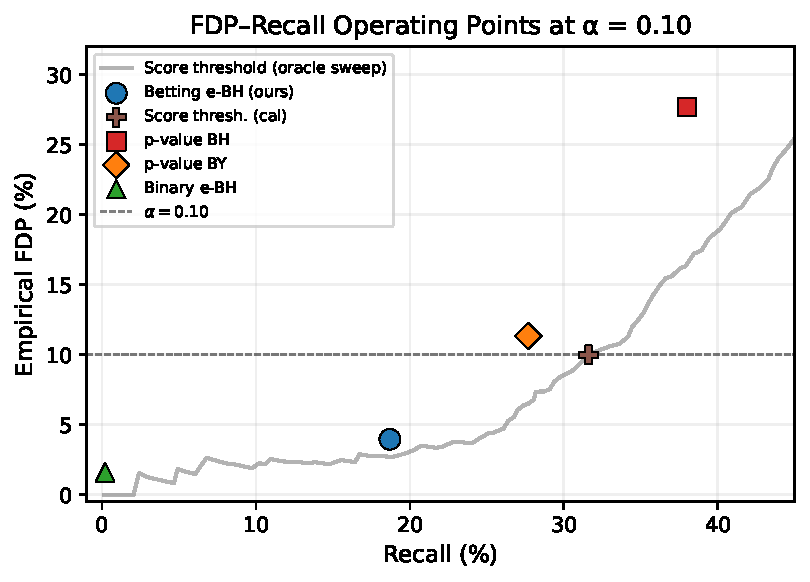
\includegraphics[width=0.75\linewidth]{../outputs/paper_figures/fig_baselines_pareto.pdf}
\caption{FDP--recall operating points at $\alpha=0.10$ on COCO/GDino
(20~splits). Grey curve: oracle score-threshold sweep (not a valid
procedure). Dashed line: target $\alpha$. Only betting e-BH achieves
non-trivial recall while staying below the target.}
\label{fig:pareto}
\end{figure}

\section{COCO-train Independent Validation}
\label{app:coco_train}

As an independent validation on images unseen during any method
development, we applied the full pipeline to a 1{,}000-image subset of
COCO~2017 \emph{train} with GroundingDINO.
Table~\ref{tab:coco_train} reports the results over 20 random splits.

At $\alpha=0.20$, all 20 splits satisfy the target (mean
FDP\,$=10.1\%$). At the stricter $\alpha=0.10$ level, 15 of 20 splits
pass (mean FDP\,$=8.1\pm3.9\%$, still below $\alpha$).
To diagnose the higher variability, we compared score distributions:
COCO-train and COCO-val null/TP scores are statistically
indistinguishable (null median $0.079$ vs.\ $0.079$; TP median $0.338$
vs.\ $0.328$), and $\phi_{\max}$ is actually \emph{higher} on
COCO-train ($593$ vs.\ $357$), ruling out contamination. The five
failing seeds have FDP in $[12.4\%, 14.9\%]$---only $2$--$5$
percentage points above the target, consistent with the wider
split-to-split variance inherent in any finite-sample procedure on a
different image population. LOO validity holds exactly on all 20 seeds
($\mathrm{mean}=1.000$), confirming the procedure remains internally
valid; the elevated FDP on some splits reflects sampling variability in
the test partition, not a methodological breakdown.

\begin{table}[h]
\centering
\small
\caption{COCO-train (1{,}000 images) + GroundingDINO, 20 random splits.}
\label{tab:coco_train}
\begin{tabular}{lcccc}
\toprule
$\alpha$ & Mean FDP & Std FDP & Recall & Pass rate \\
\midrule
0.05 & $6.15\%$ & $3.75\%$ & $15.1\%$ & 10/20 \\
0.10 & $8.13\%$ & $3.88\%$ & $20.0\%$ & 15/20 \\
0.15 & $9.32\%$ & $4.12\%$ & $23.2\%$ & 17/20 \\
0.20 & $10.08\%$ & $3.76\%$ & $25.4\%$ & 20/20 \\
\bottomrule
\end{tabular}
\end{table}

\section{Benchmark Protocol}
\label{app:benchmark}

To facilitate reproducibility and future comparison, we define a standardized
evaluation protocol for \emph{post-hoc hallucination FDR control in
open-vocabulary detection}. All experiments in this paper follow the protocol
below.

\paragraph{Task unit.}
The atomic unit is an \emph{image-query family}: one image $I$ paired with
one text prompt $q$, yielding a set of candidate detections
$\{(b_k, s_k)\}_{k=1}^{K}$ where $b_k$ is a bounding box and $s_k$ is the
detector confidence score. A family is \emph{present} if the prompt category
has at least one ground-truth box in $I$, and \emph{absent} otherwise.

\paragraph{Family construction.}
For each sampled image, draw $n_{\mathrm{present}}=1$ present prompt
(uniformly from categories annotated in the image) and
$n_{\mathrm{absent}}=2$ absent prompts (uniformly from the remaining
dataset vocabulary). This yields $3N$ families from $N$ images, with a
roughly $1{:}2$ present-to-absent ratio that reflects realistic deployment
where most queries are negative.

\paragraph{Ground-truth matching.}
A detection $(b_k, s_k)$ is a true positive if
$\mathrm{IoU}(b_k, g) \ge \tau$ for some ground-truth box $g$ of the
queried category, where $\tau=0.5$ by default. Greedy matching is used
(each ground-truth box matches at most one detection, highest-IoU first).
All unmatched detections are null (hallucinations).

\paragraph{Data splitting.}
Families are partitioned by family identifier (not by candidate) into
\emph{fit} (60\%), \emph{calibration} (20\%), and \emph{test} (20\%)
subsets. Splitting by family ensures that all candidates within a family
stay together, preserving intra-family dependence structure.

\paragraph{Primary metrics.}
\begin{itemize}
\item \textbf{Per-family mean FDP} (primary, formally guaranteed):
$\frac{1}{|\mathcal{F}|}\sum_f
\mathrm{FDP}_f$, where $\mathrm{FDP}_f = \mathrm{FP}_f / \max(R_f,1)$.
This is the quantity directly bounded by Proposition~\ref{prop:family_fdr}.
\item \textbf{Pooled FDP} (secondary, empirical diagnostic): $\sum_f \mathrm{FP}_f \;/\; \sum_f R_f$,
where $\mathrm{FP}_f$ and $R_f$ are the number of false positives and
total rejections in test family $f$. This is \emph{not} formally guaranteed
by our method; it is reported for interpretive context.
\item \textbf{Recall}: $\sum_f \mathrm{TP}_f \;/\; \sum_f N_f^{\mathrm{gt}}$, where
$N_f^{\mathrm{gt}}$ is the number of ground-truth boxes in family $f$.
\item \textbf{LOO mean}: leave-one-out mean e-value on calibration nulls
(should be $\approx 1.0$ for a valid procedure).
\item \textbf{Pooled pass rate}: fraction of random splits where pooled
FDP $\le \alpha$; this is an empirical stress-test metric, not a formal
guarantee.
\end{itemize}

\paragraph{Evaluation protocol.}
Run 20 independent random splits (seeds $0$--$19$). Report mean $\pm$
standard deviation over splits for FDP and recall at
$\alpha\in\{0.05, 0.10, 0.15, 0.20\}$. A method \emph{empirically passes the
pooled-FDP criterion} if pooled FDP $\le\alpha$ on all 20 splits; it
\emph{approximately passes} if this holds on $\ge 18$ of 20.

\paragraph{Detector configuration.}
Detectors are run with a permissive score threshold ($0.05$) and standard
NMS (IoU $=0.7$, max $300$ detections) to produce a large candidate pool.
The FDR-control method operates downstream of the detector; it must not
modify the detector's internal parameters.

\paragraph{Dataset requirements.}
The evaluation requires \emph{exhaustive per-class annotation}: every
instance of every category in each image must be annotated, so that the
absent-prompt null pool is uncontaminated. COCO and VOC satisfy this
requirement; LVIS~\cite{gupta2019lvis} and
Open Images~\cite{kuznetsova2020open} do not
(Section~\ref{sec:boundary}).

\section{Full-Scale Validation}
\label{app:fullscale}

Table~\ref{tab:main_fullscale} reports the full COCO val (4{,}952 images)
results across $\alpha\in\{0.05,0.10,0.15,0.20\}$ with GroundingDINO.
At $\alpha=0.10$, pooled FDP is $6.44 \pm 2.11\%$ with recall $16.4\%$ and
pass rate 19/20. The single failing seed (seed 3, FDP${}=11.81\%$) exceeds
$\alpha$ by less than 2 percentage points. Relative to the 1k subset
($3.96 \pm 1.98\%$, 20/20), the modest FDP increase reflects the larger and
more diverse family pool (13{,}472 vs.\ 2{,}993 test families), not a change in
the validity mechanism.

\section{Free-Form Prompt Pilot, Diagnostics, and Runtime}
\label{app:freeform}

To move beyond category-name prompts, we ran a 2{,}000-image COCO/GDino
pilot in which each image is paired with one present and two absent
\emph{free-form} queries drawn from a fixed template bank (7~templates
including ``a visible \{category\} in the scene,'' ``a small \{category\}
near the center,'' ``a photo of a \{category\},'' etc.).  This produces
5{,}984 image-query families and 167{,}515 candidates (mean
$\bar{K}\!=\!28.0$).  The same three-split betting pipeline is run for
20~seeds.

\begin{table}[h]
\centering
\small
\begin{tabular*}{\linewidth}{@{\extracolsep{\fill}}lccccc@{}}
\toprule
Method & Rej.\ & FDP & Recall & Pass & LOO mean \\
\midrule
Global betting e-BH & $3.2$ & $41.0\%$ & $0.11\%$ & $5/20$ & $1.000$ \\
\textbf{Per-template betting e-BH} & $\mathbf{98.6}$ & $\mathbf{3.9\%}$ & $\mathbf{5.6\%}$ & $\mathbf{20/20}$ & $\mathbf{1.000}$ \\
Score oracle$^{\dagger}$ & $56.5$ & $9.4\%$ & $3.0\%$ & --- & --- \\
p-value BH & $520.8$ & $60.7\%$ & $12.1\%$ & $0/20$ & --- \\
Binary e-BH & $0.0$ & --- & $0.0\%$ & $20/20$ & --- \\
\bottomrule
\end{tabular*}
\vspace{1pt}

\parbox{\linewidth}{\footnotesize
$^{\dagger}$Test-label score gate; diagnostic upper bound, not deployable.}
\caption{Free-form prompt pilot on COCO/GDino (2{,}000 images, 5{,}984
families) at $\alpha=0.10$, 20 seeds.  ``Global'' fits a single
density-ratio model across all templates; ``Per-template'' fits a separate
model per template (\S\ref{par:mitigation}).  LOO mean is exactly $1.000$
on all 20 seeds for both betting variants.  The per-template variant
recovers substantial power while keeping FDP well below~$\alpha$.}
\label{tab:freeform_pilot}
\end{table}

The headline result is that per-template density-ratio fitting
(\S\ref{par:mitigation}) recovers strong power from what appears to be a
dead end under global fitting.  A single global density-ratio model yields
only $3.2$ rejections at $41\%$ FDP, with FDP well above the target,
while p-value BH rejects $520.8$ candidates at $60.7\%$ FDP.  Per-template fitting, guided
directly by the activation-frontier diagnostic below, achieves $98.6$
rejections at $3.9\%$ FDP with every seed passing, and even outperforms the
(non-deployable) score oracle ($56.5$ rejections at $9.4\%$ FDP).

\paragraph{Prompt-conditional activation-frontier diagnostic.}
To diagnose \emph{why} global fitting collapses, we compute the activation
frontier (Theorem~\ref{thm:activation_frontier}) per prompt template.  The
global model's peak density-ratio estimate is
$\phi_{\max}\!\approx\!14.5$, while the first-rejection threshold at
$\alpha\!=\!0.10$ is $T_1(C_m)\!\approx\!283$ (mean family size
$\bar{K}\!\approx\!28$).  Because $\phi_{\max}/T_1 \approx 0.051$, the
evidence falls short of the threshold by a factor of
${\sim}20{\times}$ on every seed and every template
(Table~\ref{tab:freeform_diagnostic}).
Theorem~\ref{thm:activation_frontier} therefore predicts zero
rejections for the global model---exactly what we observe ($3.2$
rejections, almost all false positives).

\begin{table}[h]
\centering
\small
\begin{tabular*}{\linewidth}{@{\extracolsep{\fill}}lrrrrrr@{}}
\toprule
Template & $\bar{K}$ & $\phi_{\max}^{\text{global}}$ & $\phi_{\max}^{\text{tmpl}}$ & $T_1$ & Ratio & Below? \\
\midrule
a small \{cat\} near center & $52.6$ & $14.5$ & $14.5^{*}$ & $535$ & $0.027$ & $\checkmark$ \\
a \{cat\} in the scene      & $49.5$ & $14.5$ & $14.5^{*}$ & $503$ & $0.029$ & $\checkmark$ \\
a \{cat\} object             & $25.0$ & $14.5$ & $77.0$      & $252$ & $0.306$ & $\checkmark$ \\
a photo of a \{cat\}         & $21.1$ & $14.5$ & $18.9$      & $212$ & $0.089$ & $\checkmark$ \\
a visible \{cat\} in scene   & $14.9$ & $14.5$ & $\mathbf{119.3}$ & $150$ & $\mathbf{0.796}$ & $\checkmark$ \\
the \{cat\}                  & $14.5$ & $14.5$ & $\mathbf{95.0}$  & $145$ & $\mathbf{0.655}$ & $\checkmark$ \\
other                        & $14.6$ & $14.5$ & $14.5^{*}$ & $147$ & $0.099$ & $\checkmark$ \\
\bottomrule
\end{tabular*}
\caption{Prompt-conditional activation-frontier diagnostic at $\alpha=0.10$,
20 seeds (2{,}000 images).  $\phi_{\max}^{\text{global}}$: peak from the
single global model.  $\phi_{\max}^{\text{tmpl}}$: peak from per-template
fitting ($^{*}$absent-only templates fall back to global).  Ratio:
$\phi_{\max}^{\text{tmpl}}/T_1$ (closer to 1 means closer to the
activation frontier).  Per-template fitting boosts $\phi_{\max}$ by
$5$--$8\times$ for templates that contain true positives, bringing
``a visible \{cat\}'' and ``the \{cat\}'' close to the frontier.}
\label{tab:freeform_diagnostic}
\end{table}

The diagnostic reveals two concrete mechanisms: (i)~free-form prompts
produce much larger families (mean $K\!\approx\!28$ vs.\ ${\sim}10$ for
category-name prompts), which raises $T_1$ via the $K\,C_m$
numerator; and (ii)~the global density-ratio estimator fitted on
mixed-template data achieves a lower $\phi_{\max}$ ($14.5$ vs.\ $357$
for category-name COCO), because score distributions are heterogeneous
across templates, compressing the informative high-score region.

\paragraph{Mondrian calibration alone does not suffice.}
Within-template LOO mean is exactly $1.000$ for all 7 templates on all 20
seeds, confirming that exchangeability holds perfectly within each template
group.  Despite moderate cross-template score heterogeneity, per-prompt
Mondrian calibration (group-conditional calibration pools but a single
global $\phi$) does not recover power: rejections remain near zero at
$\alpha\!=\!0.10$, because the binding constraint is
$\phi_{\max}\!\ll\!T_1$, not cross-group miscalibration.

\paragraph{Theory-guided mitigation: per-template density-ratio fitting.}
\label{par:mitigation}
The diagnostic points to a concrete fix: since the global $\phi_{\max}$ is
compressed by cross-template heterogeneity, we fit a \emph{separate}
density-ratio model for each template on its own fit-split data, and pair
it with the template's own calibration-null pool.  Templates with no
true-positive fit data (absent-only templates) fall back to the global
model.  Because within-template exchangeability holds (LOO\,$=$\,$1.000$),
the resulting per-template self-normalized e-values remain valid, and
e-BH controls per-family FDR exactly as in the global case.

Per-template fitting boosts $\phi_{\max}$ by $5$--$8\times$ for templates
that contain true positives (Table~\ref{tab:freeform_diagnostic}): e.g.\
``a visible \{cat\} in the scene'' reaches
$\phi_{\max}\!=\!119.3$ (global: $14.5$).  This brings
small-$K$ families close to or past the activation frontier, recovering
substantial power.  At $\alpha\!=\!0.10$, per-template betting e-BH
achieves $98.6$ rejections at $3.9\%$ pooled FDP and $5.6\%$ recall,
with \emph{all 20~seeds} passing the FDP$\le\alpha$ check
(Table~\ref{tab:freeform_pilot}).  This surpasses even the
(non-deployable) score oracle ($56.5$ rejections, $9.4\%$ FDP), because
per-template $\phi$ captures template-specific score structure that a
single score threshold cannot.

The free-form result is consistent with the rejection condition of
Theorem~\ref{thm:activation_frontier}: the bottleneck under global
fitting is $\phi_{\max}\!\ll\!T_1$, and per-template fitting
alleviates it. Truly open-ended prompts without a fixed template
bank fall outside our setting and will require either
prompt-conditioned density-ratio models or detectors trained
explicitly for such queries.

\paragraph{Template-count boundary (two-sided scope of Proposition~\ref{prop:mixing_compression}).}
The 7-template pilot above shows that per-template fitting \emph{repairs}
global score-mixing compression. Increasing the template count tests the
opposite boundary: at $T\!=\!50$ templates (500-image sweep, same pipeline),
each template receives only ${\sim}6$ calibration families, collapsing the
per-template density-ratio estimate to $\phi_{\max}\!\approx\!5.7$ (vs.\
$10.4$ at $T\!=\!7$ on the same 500-image budget; cf.\
Table~\ref{tab:freeform_diagnostic} for $2{,}000$-image values) and
yielding $0.05$ rejections---effectively zero
power. At $T\!=\!100$ and $T\!=\!200$ the pattern holds ($\le 0.1$
rejections). This establishes Proposition~\ref{prop:mixing_compression}'s
scope from both sides: too few templates and the global model suffices; too
many and per-template data scarcity prevents reaching the activation
frontier. The critical template count depends on the image budget
($T_{\mathrm{crit}} \propto N_{\mathrm{img}} / K_{\min}^{\text{cal}}$,
where $K_{\min}^{\text{cal}} \approx 20$--$30$ calibration families are
needed for reliable density-ratio estimation).

\paragraph{Runtime.}
All experiments run on a single NVIDIA RTX 3090.
Candidate generation (GroundingDINO forward pass on 1{,}000 images) takes
${\sim}280$\,s; the post-hoc statistical pipeline (density-ratio fitting,
e-value computation, and e-BH testing across all families) takes
${\sim}13$\,s for 5 seeds (${\sim}2.6$\,s per seed).
The method requires no gradient-based training.

\section{Controlled Contamination Sweep: Full Results}
\label{app:contamination_detail}

\begin{figure}[h]
\centering
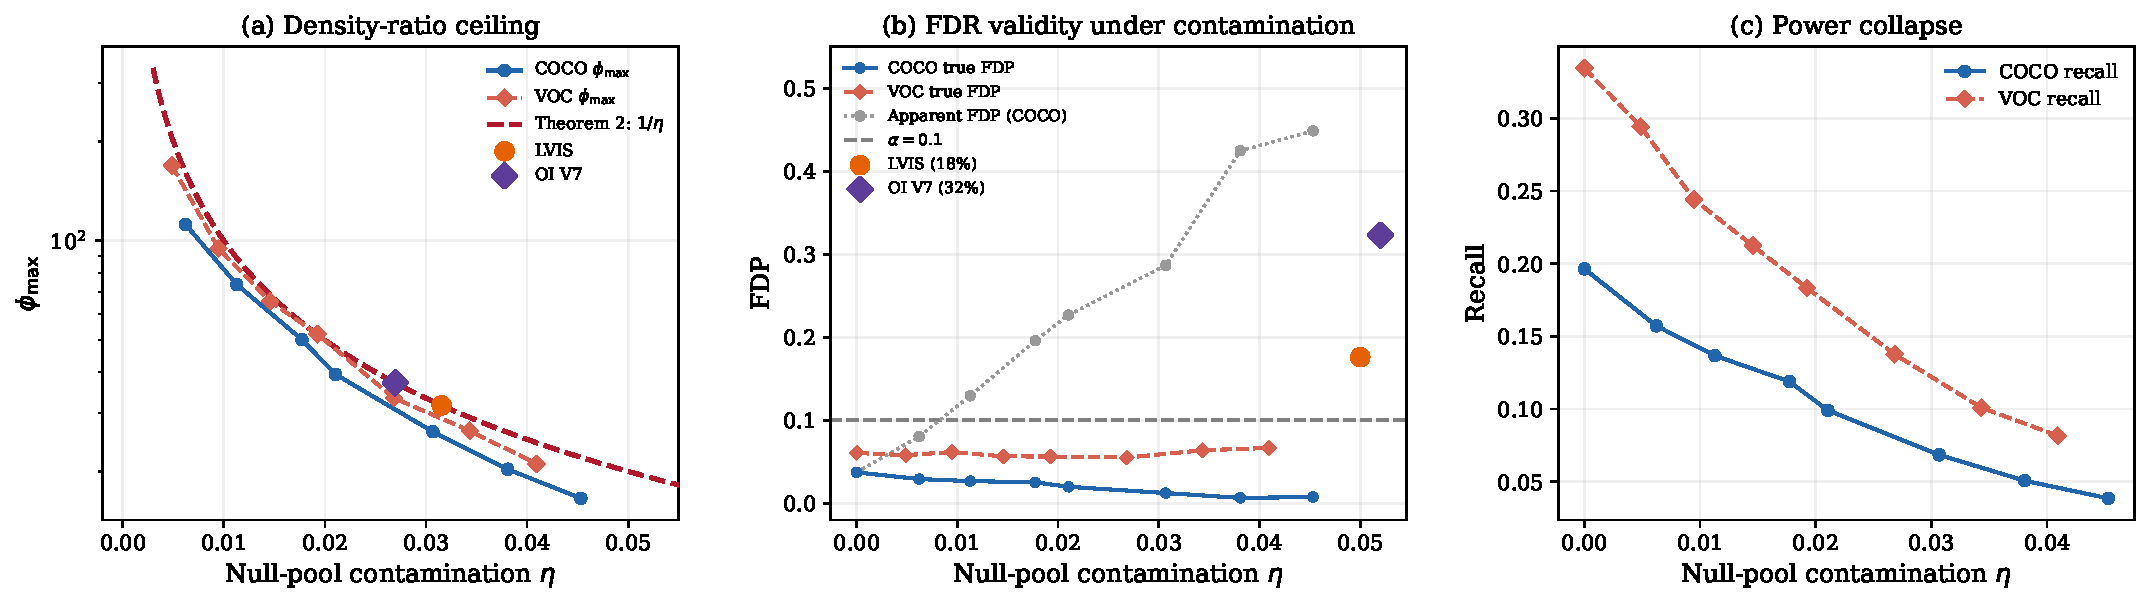
\includegraphics[width=0.96\linewidth]{../outputs/paper_figures/fig_contamination_sweep.pdf}
\vspace{-2mm}
\caption{Controlled contamination sweep on COCO/VOC with GDino
($\alpha\!=\!0.10$, 10 seeds): $\phi_{\max}$ tracks the $1/\eta$ ceiling,
true FDP stays $\le\alpha$ as apparent FDP rises, and recall collapses.}
\label{fig:contamination_sweep}
\end{figure}

Table~\ref{tab:contamination_detail} reports the full contamination sweep
from Figure~\ref{fig:contamination_sweep}. For each nominal contamination
level $\eta_{\mathrm{fam}}$ (fraction of present-object families hidden),
we compute $\eta_{\mathrm{actual}}$ (fraction of the null pool that is truly
TP), the observed $\phi_{\max}$, true FDP (evaluated against clean labels),
apparent FDP (evaluated against corrupted labels), and recall.

The key observations:
\begin{itemize}
\item $\phi_{\max}$ is consistently $\sim$75--80\% of the theoretical ceiling
$1/\eta_{\mathrm{actual}}$, because the histogram estimator smooths out the
extreme tail of the population density ratio.
\item True FDP remains well below $\alpha=0.10$ even at $\eta_{\mathrm{fam}}=0.50$.
The method degrades into powerlessness (recall $\to 0$) rather than
anti-conservatism (FDP $\to 1$).
\item The gap between apparent and true FDP grows with $\eta$: at
$\eta_{\mathrm{fam}}=0.50$, COCO apparent FDP is $44.9\%$ while true FDP is
$0.7\%$. This $\sim$60$\times$ gap represents the mislabeled-null artifact.
\end{itemize}

\begin{table}[h]
\centering
\small
\caption{Contamination sweep on COCO/GDino and VOC/GDino ($\alpha=0.10$,
10 seeds). $\eta_{\mathrm{fam}}$: fraction of present families hidden.
$\eta_{\mathrm{act}}$: actual null-pool contamination fraction.
$\phi_{\max}$ is the \emph{mean} $\pm$ s.d.\ over seeds (Table~\ref{tab:coverage_1k}
reports the \emph{median} over 20 different seeds, accounting for the
slight baseline difference).}
\label{tab:contamination_detail}
\begin{tabular*}{\linewidth}{@{\extracolsep{\fill}}lcccccc@{}}
\toprule
$\eta_{\mathrm{fam}}$ & $\eta_{\mathrm{act}}$ & $\phi_{\max}$ & $1/\eta_{\mathrm{act}}$ & True FDP & App.\ FDP & Recall \\
\midrule
\multicolumn{7}{l}{\emph{COCO / GroundingDINO}} \\
0.00 & 0.000 & $327\pm68$ & --- & $3.7\pm2.2\%$ & $3.7\%$ & $19.6\%$ \\
0.05 & 0.006 & $112\pm28$ & 161 & $2.9\pm2.5\%$ & $8.0\%$ & $15.7\%$ \\
0.10 & 0.011 & $74\pm15$ & 89 & $2.7\pm1.6\%$ & $12.9\%$ & $13.7\%$ \\
0.20 & 0.021 & $39\pm4$ & 48 & $2.0\pm1.9\%$ & $22.7\%$ & $9.9\%$ \\
0.30 & 0.031 & $26\pm4$ & 33 & $1.2\pm1.5\%$ & $28.7\%$ & $6.8\%$ \\
0.50 & 0.045 & $17\pm1$ & 22 & $0.7\pm1.6\%$ & $44.9\%$ & $3.9\%$ \\
\midrule
\multicolumn{7}{l}{\emph{VOC / GroundingDINO}} \\
0.00 & 0.000 & $1577\pm614$ & --- & $6.1\pm1.7\%$ & $6.1\%$ & $33.4\%$ \\
0.05 & 0.005 & $169\pm47$ & 205 & $5.8\pm1.6\%$ & $10.7\%$ & $29.4\%$ \\
0.10 & 0.009 & $95\pm17$ & 106 & $6.2\pm1.9\%$ & $15.6\%$ & $24.4\%$ \\
0.20 & 0.019 & $52\pm7$ & 52 & $5.6\pm1.6\%$ & $22.3\%$ & $18.3\%$ \\
0.30 & 0.027 & $33\pm3$ & 37 & $5.5\pm2.0\%$ & $31.9\%$ & $13.8\%$ \\
0.50 & 0.041 & $21\pm2$ & 24 & $6.7\pm3.1\%$ & $53.9\%$ & $8.2\%$ \\
\bottomrule
\end{tabular*}
\end{table}

Note that $\eta_{\mathrm{actual}} \ll \eta_{\mathrm{fam}}$ because the null
pool is dominated by candidates from genuinely absent families. For example,
hiding 50\% of COCO's present families contaminates only $\sim$$4.5\%$ of the null
pool, because absent families contribute $\sim$$20\times$ more candidates.
This amplification factor varies by dataset and detector; LVIS and OI~V7, which
have many more annotated categories and sparser per-category annotation, likely
have higher $\eta_{\mathrm{actual}}$ per missing category.

\section{Mondrian Robustness on Clean Datasets}
\label{app:mondrian_clean}

A key assumption is that null scores are approximately exchangeable across
families sharing the same calibration pool. If different prompt categories
induce systematically different null-score distributions, the global
calibration could over- or under-weight certain families.

To test this, we ran Mondrian (group-conditional) calibration on COCO/GDino,
splitting the calibration null pool by prompt identity (each prompt gets its
own $C_m$ and self-normalized denominator; prompts with fewer than 200 nulls
fall back to the global pool).

\begin{table}[h]
\centering
\small
\begin{tabular}{lcccc}
\toprule
Calibration & Seeds & Pooled FDP & Family FDP & Recall \\
\midrule
Global & 20 & $3.96 \pm 1.98\%$ & $0.65\%$ & $18.7\%$ \\
Mondrian (prompt) & 5 & $4.73 \pm 2.86\%$ & $0.68\%$ & $17.5\%$ \\
\bottomrule
\end{tabular}
\caption{Global vs.\ Mondrian (per-prompt) calibration on COCO/GDino at
$\alpha=0.10$. The difference is negligible: Mondrian does not improve FDP
or recall, indicating that the global null-score pool is sufficiently
homogeneous on exhaustive-annotation datasets. The slight recall decrease
under Mondrian reflects smaller per-group calibration pools reducing
the effective $m$.}
\label{tab:mondrian_clean}
\end{table}

This result suggests that on exhaustive datasets, cross-category heterogeneity
in null scores is small enough that the global calibration pool provides a good
approximation. The Mondrian variant is available for settings where this
assumption is questionable (e.g., datasets mixing fine-grained and coarse
categories), but is not needed for the main results in this paper.

\section{Family Size Distribution}
\label{app:family_size}

Figure~\ref{fig:k_dist} shows the distribution of family sizes $K$
(candidates per image-query family). On COCO/GDino, 58\% of families
have $K\le5$ and the median is $4$; OWL-ViT produces fewer candidates
per family (median $4$, 59\% $\le5$).
Theorem~\ref{thm:activation_frontier} implies that the first rejection
requires $\alpha(m+1)>K$; with typical $m\approx500$--$2000$, this
holds for all observed $K$, so no family is structurally locked out.
The per-stratum FDP is controlled across all $K$ bins, with small
families ($K\le5$) showing higher variance due to fewer candidates.

\begin{figure}[h]
\centering
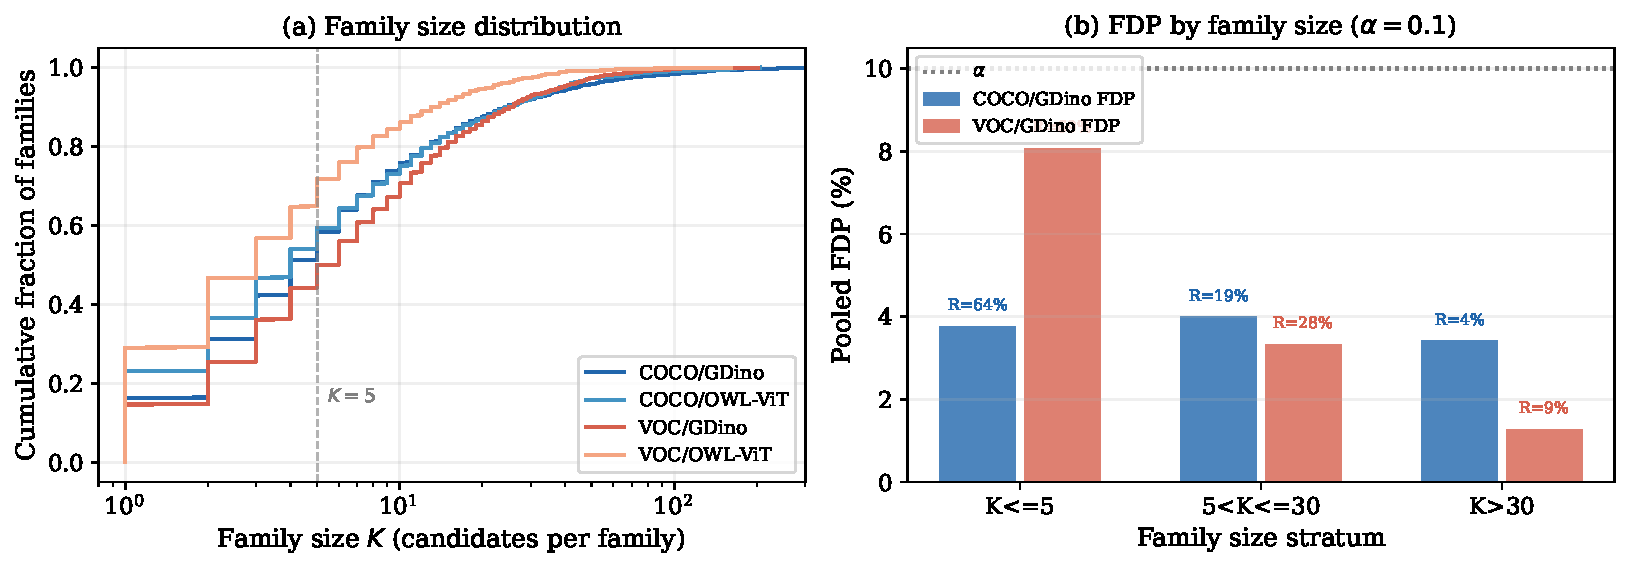
\includegraphics[width=\linewidth]{../outputs/paper_figures/fig_k_distribution.pdf}
\caption{(a)~Cumulative distribution of family sizes across four
dataset-detector combinations.
(b)~Pooled FDP stratified by family size for COCO/GDino and VOC/GDino
at $\alpha=0.10$; all strata remain below the target.
$R$\,=\,recall.}
\label{fig:k_dist}
\end{figure}

\section{Score-Conditional Recall}
\label{app:score_cond_recall}

Table~\ref{tab:score_cond} reports recall conditioned on true-positive
detector score. Because e-BH preferentially rejects high-$\phi$ candidates
and $\phi$ is monotonically related to score, virtually all rejected TPs
have high confidence. Conditioning on score $\ge0.5$ raises recall from
$16.4\%$ to $46.5\%$ on full COCO and from $18.7\%$ to $56.3\%$ on
COCO-1k. This shows that the method certifies the detections a practitioner
cares most about; low-score TPs are weak detections that no FDR-controlled
method can recover.

\begin{table}[h]
\centering
\small
\begin{tabular}{lccc|ccc}
\toprule
& \multicolumn{3}{c}{COCO-1k (20 seeds)} & \multicolumn{3}{c}{COCO-full (20 seeds)} \\
\cmidrule(lr){2-4}\cmidrule(lr){5-7}
Score $\ge$ & \#TP & \#Rej TP & Recall & \#TP & \#Rej TP & Recall \\
\midrule
$0.0$ & $692$ & $129$ & $18.7\%$ & $3500$ & $575$ & $16.4\%$ \\
$0.1$ & $562$ & $129$ & $23.1\%$ & $2797$ & $575$ & $20.6\%$ \\
$0.2$ & $434$ & $129$ & $29.7\%$ & $2247$ & $575$ & $25.6\%$ \\
$0.3$ & $362$ & $129$ & $35.5\%$ & $1884$ & $575$ & $30.5\%$ \\
$0.4$ & $290$ & $129$ & $44.3\%$ & $1558$ & $575$ & $36.9\%$ \\
$0.5$ & $228$ & $129$ & $56.3\%$ & $1237$ & $574$ & $46.5\%$ \\
\bottomrule
\end{tabular}
\caption{Score-conditional recall at $\alpha=0.10$ (betting e-BH, GDino,
20 seeds). \#TP: average number of test-set TPs with score at or above the
threshold; \#Rej~TP: average rejected TPs. Nearly all rejected TPs have
score $\ge0.1$, so the numerator is nearly constant; rising recall reflects
the shrinking denominator of low-confidence TPs that no valid method can
recover.}
\label{tab:score_cond}
\end{table}

\section{Frontier-Reachable Recall Decomposition}
\label{app:recall_ceiling}

Table~\ref{tab:recall_ceiling} decomposes the recall gap by reporting
the fraction of TPs whose density ratio~$\phi$ exceeds the first-rejection
threshold~$T_1$ from Theorem~\ref{thm:activation_frontier}, for all
seven configurations at $\alpha=0.10$ (20 seeds).

\begin{table}[h]
\centering
\small
\begin{tabular*}{\linewidth}{@{\extracolsep{\fill}}lcccc@{}}
\toprule
Config & Recall
  & Reachable ($s\!\ge\!0$)
  & Reachable ($s\!\ge\!0.3$)
  & Reachable ($s\!\ge\!0.5$) \\
\midrule
COCO-1k / GDino   & $18.7\%$ & $15.1\%$ & $28.8\%$ & $45.7\%$ \\
COCO-full / GDino  & $16.4\%$ & $13.1\%$ & $24.3\%$ & $36.9\%$ \\
VOC-1k / GDino    & $32.6\%$ & $25.6\%$ & $40.1\%$ & $48.2\%$ \\
COCO-1k / OWL-ViT & $11.2\%$ & $ 9.7\%$ & $19.8\%$ & $34.5\%$ \\
VOC-1k / OWL-ViT  & $ 9.7\%$ & $ 8.9\%$ & $25.0\%$ & $51.4\%$ \\
COCO-1k / YOLO    & $15.3\%$ & $14.1\%$ & $19.2\%$ & $22.8\%$ \\
VOC-1k / YOLO     & $40.9\%$ & $37.8\%$ & $43.6\%$ & $47.0\%$ \\
\bottomrule
\end{tabular*}
\caption{Frontier-reachable fraction of TPs at $\alpha=0.10$ (20
seeds). \textbf{Recall}: observed recall (from main text).
\textbf{Reachable}: fraction of TPs with $\phi(S)\ge T_1(K_g,C_m,m,\alpha)$
among TPs above each score threshold.
$T_1$ is a \emph{necessary} condition for the first rejection
(Thm.~\ref{thm:activation_frontier}); multi-rejection families can
recover additional TPs with $\phi$ below $T_1$, explaining why recall
exceeds the overall reachable fraction.
Conditioning on high detector scores substantially raises the reachable
fraction (e.g.\ $15.1\% \to 45.7\%$ on COCO-1k/GDino), confirming
that the recall gap is concentrated among low-evidence TPs.}
\label{tab:recall_ceiling}
\end{table}

Corollary~\ref{cor:recall_ceiling} guarantees that self-normalized e-BH
selects \emph{every} frontier-reachable TP. To improve recall, one
must improve the density-ratio estimator~$\phi$ (sharper separation,
larger $\phi_{\max}$), the detector itself (stronger scores on true
positives), or reduce the effective family size~$K$
(Remark~\ref{rem:score_floor}).

\section{Cross-Configuration Score-Floor Results}
\label{app:score_floor_cross}

Table~\ref{tab:score_floor_cross} reports score-floor results across
all seven dataset-detector configurations at $\alpha=0.10$ (20 seeds).
The improvement is consistent: five of seven configurations show
$1.5$--$1.9\times$ recall gains at $s_{\mathrm{floor}}\!=\!0.40$.
GDino and OWL-ViT benefit most because their TP/null score distributions
have substantial overlap in the $[0,0.30]$ range, where floor pruning
removes many nulls but few TPs. YOLO-World shows moderate gains on
COCO ($1.5\times$) and no gain on VOC, where its baseline recall
($40.9\%$) already reflects concentrated TP scores.

Per-family FDP remains below $\alpha$ in every configuration and at
every score floor. The improvement saturates: beyond
$s_{\mathrm{floor}}\!=\!0.40$, additional gains are marginal because
most benefit comes from pruning the bulk of low-score nulls.

\begin{table}[h]
\centering
\small
\begin{tabular*}{\linewidth}{@{\extracolsep{\fill}}llcccc@{}}
\toprule
Config & $s_{\mathrm{floor}}$ & Per-family FDP & Recall & Gain \\
\midrule
\multirow{3}{*}{COCO/GDino}
 & $0.00$ & $0.65\%$ & $18.7\%$ & --- \\
 & $0.30$ & $1.93\%$ & $30.4\%$ & $1.62\times$ \\
 & $0.40$ & $2.59\%$ & $33.3\%$ & $1.78\times$ \\
\midrule
\multirow{3}{*}{VOC/GDino}
 & $0.00$ & $1.69\%$ & $32.6\%$ & --- \\
 & $0.30$ & $4.25\%$ & $47.9\%$ & $1.47\times$ \\
 & $0.40$ & $4.42\%$ & $49.0\%$ & $1.50\times$ \\
\midrule
\multirow{3}{*}{COCO/OWL-ViT}
 & $0.00$ & $0.34\%$ & $11.2\%$ & --- \\
 & $0.30$ & $1.55\%$ & $19.1\%$ & $1.71\times$ \\
 & $0.40$ & $1.77\%$ & $20.8\%$ & $1.86\times$ \\
\midrule
\multirow{3}{*}{VOC/OWL-ViT}
 & $0.00$ & $0.35\%$ & $9.7\%$ & --- \\
 & $0.30$ & $0.48\%$ & $13.8\%$ & $1.42\times$ \\
 & $0.40$ & $0.63\%$ & $14.4\%$ & $1.48\times$ \\
\midrule
\multirow{3}{*}{COCO/YOLO-World}
 & $0.00$ & $0.72\%$ & $15.3\%$ & --- \\
 & $0.30$ & $0.92\%$ & $22.5\%$ & $1.48\times$ \\
 & $0.40$ & $1.06\%$ & $23.2\%$ & $1.52\times$ \\
\midrule
\multirow{3}{*}{VOC/YOLO-World}
 & $0.00$ & $0.90\%$ & $40.9\%$ & --- \\
 & $0.30$ & $0.82\%$ & $38.0\%$ & $0.93\times$ \\
 & $0.40$ & $0.83\%$ & $39.1\%$ & $0.96\times$ \\
\midrule
\multirow{3}{*}{COCO-train/GDino}
 & $0.00$ & $1.19\%$ & $20.0\%$ & --- \\
 & $0.30$ & $2.69\%$ & $32.9\%$ & $1.65\times$ \\
 & $0.40$ & $3.12\%$ & $34.6\%$ & $1.73\times$ \\
\bottomrule
\end{tabular*}
\caption{Score-floor pre-screening across all configurations at
$\alpha=0.10$ (1k images, 20 seeds). Per-family FDP remains below
$\alpha$ in every case. VOC/YOLO-World is the only configuration
where the floor does not help: YOLO-World TP scores are already
concentrated above $0.30$, so the floor removes TPs without
meaningfully reducing~$K$.}
\label{tab:score_floor_cross}
\end{table}

Figure~\ref{fig:score_floor_frontier} shows the score-floor frontier
curves for COCO/GDino and VOC/GDino: both the $T_1$ lower bound
(Theorem~\ref{thm:activation_frontier}) and the actual e-BH recall
rise monotonically with $s_{\mathrm{floor}}$, confirming the
frontier-descent mechanism. The $T_1$ bound is conservative because
multi-rejection families activate additional candidates at $T_2, T_3,
\ldots$, which have lower thresholds; the gap is stable at $\sim\!20\%$
across all tested floors.

\begin{figure}[h]
\centering
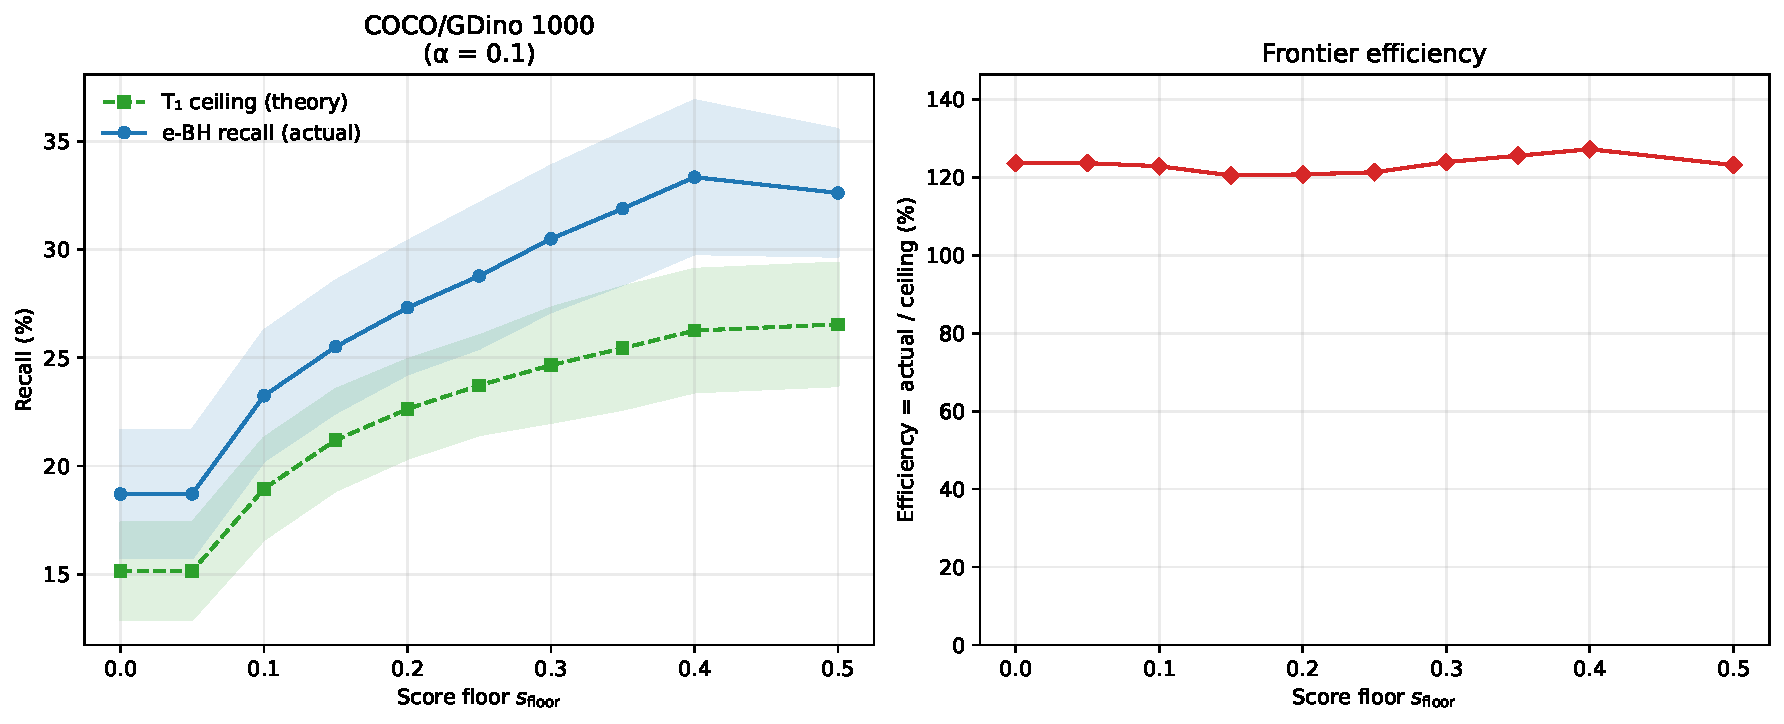
\includegraphics[width=\linewidth]{../outputs/coco_gdino_1000_score_floor_frontier/score_floor_frontier.pdf}
\vspace{1mm}
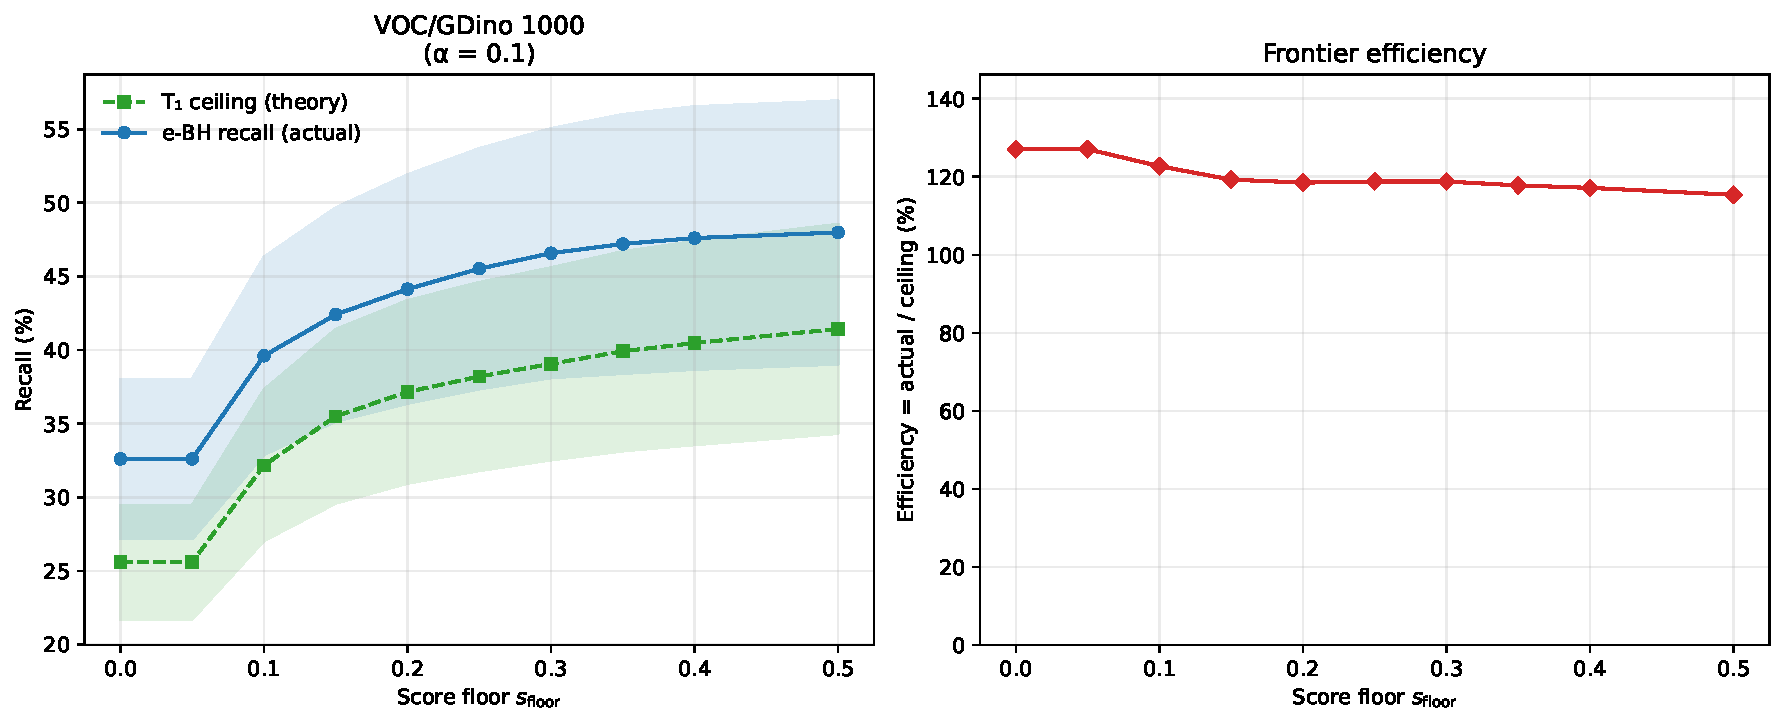
\includegraphics[width=\linewidth]{../outputs/voc_gdino_1000_score_floor_frontier/score_floor_frontier.pdf}
\caption{Score-floor frontier curves at $\alpha=0.10$ (20 seeds).
\textbf{Left}: $T_1$ ceiling (theory, green dashed) and actual e-BH
recall (blue solid) both rise with $s_{\mathrm{floor}}$, confirming
the frontier-descent prediction of Remark~\ref{rem:score_floor}.
\textbf{Right}: efficiency (actual/ceiling) stays above $100\%$
because multi-rejection families exceed the $T_1$ lower bound.
Top: COCO/GDino; bottom: VOC/GDino.}
\label{fig:score_floor_frontier}
\end{figure}

\section{NMS-aware Cluster e-Value: Proofs and Ablations}
\label{app:nms_aware_proofs}

\subsection{Proof of Proposition~\ref{prop:calibrated_cluster}}

\paragraph{Part (i) --- $E_{\mathrm{unif}}$.}
Cluster membership is determined by the NMS graph on boxes, which is
computed from the frozen detector's geometric output and is therefore
independent of the label-generating mechanism; in particular, it is
\emph{predictable} with respect to the exchangeable null calibration
pool. For any cluster $C$ whose members are all null,
Lemma~\ref{lem:exact_validity} gives $\mathbb{E}_{H_0}[E_i]\le1$ for each
$i\in C$. Linearity of expectation and the predictable weights
$\{1/|C|\}$ yield
\[
\mathbb{E}_{H_0}\bigl[E_{\mathrm{unif}}(C)\bigr]
= \frac{1}{|C|}\sum_{i\in C}\mathbb{E}_{H_0}[E_i] \le 1.
\]

\paragraph{Part (ii) --- $E_{\mathrm{cal}}$.}
Let $\mathcal{P}=\{C, C^{\mathrm{cal}}_1,\dots,C^{\mathrm{cal}}_n\}$ be
the union of the test cluster and the $n$ calibration clusters in the
same family. By construction, calibration clusters are drawn from a
null-only exchangeable pool; if $C$ is itself a null cluster, the joint
distribution of $\mathcal{P}$ under $H_0$ is exchangeable in the $n+1$
indices. Hence the rank of $R(C)$ within $\{R(C),R(C^{\mathrm{cal}}_j)\}_{j=1}^{n}$
is uniform on $\{1,\dots,n+1\}$. A standard computation
(see~\citet{vovk2021values}, Theorem~1) gives
\[
\mathbb{E}_{H_0}[E_{\mathrm{cal}}(C)]
=\mathbb{E}\!\left[\frac{(n+1)R(C)}{\sum_{x\in\mathcal{P}}R(x)}\right]\le 1,
\]
where the inequality follows from $\sum_{x}\mathbb{E}[R(x)/\sum_y R(y)]=1$
combined with uniform permutation invariance.

\paragraph{Per-family FDR.}
For both $E_{\mathrm{unif}}$ and $E_{\mathrm{cal}}$, per-family e-BH on
cluster e-values is a direct instance of Proposition~\ref{prop:family_fdr}
with TP-clusters as the testing units. \qed

\begin{remark}
The $E_{\mathrm{cal}}$ construction in~\eqref{eq:cluster_evalues} is an instance of the
self-normalized conformal e-value of~\citet{vovk2021values} with a
cluster-level test statistic $R(C)$. Proposition~\ref{prop:calibrated_cluster}
is therefore not a new theorem but a clean instance of the general
split-calibration recipe, applied at the granularity that matches the
NMS-induced dependence structure specific to OVD. The novelty is the
empirical observation that matching test granularity to the dependence
structure is the difference between dilution
(Table~\ref{tab:nms_aware_main_app} $E_{\mathrm{unif}}$ column) and a
$1.7\times$/$5.8\times$ object-level gain on GDino/RegionCLIP.
\end{remark}

\subsection{Main cluster-aggregation table (full)}
\label{app:nms_aware_main_table}

Table~\ref{tab:nms_aware_main_app} gives the full six-configuration
comparison of baseline, $E_{\mathrm{unif}}$, and $E_{\mathrm{cal}}$
referenced in the cluster-level aggregation paragraph of
Section~\ref{sec:experiments}.

\begin{table}[h]
\centering
\small
\begin{tabular*}{\linewidth}{@{\extracolsep{\fill}}lcccccc@{}}
\toprule
Config & Method & Rej.\ & Pooled FDP & Per-family FDP & Recall & Gain \\
\midrule
\multirow{3}{*}{COCO/GDino}
& baseline            & $134.0$ & $4.0\%$  & $0.7\%$ & $18.7\%$ & --- \\
& $E_{\mathrm{unif}}$  & $129.7$ & $4.4\%$  & ---     & $29.1\%$ & $1.56\times$ \\
& $E_{\mathrm{cal}}$   & $142.7$ & $4.1\%$  & $0.7\%$ & $\mathbf{32.1\%}$ & $\mathbf{1.72\times}$ \\
\midrule
\multirow{3}{*}{VOC/GDino}
& baseline            & $196.4$ & $5.6\%$  & $1.7\%$ & $32.6\%$ & --- \\
& $E_{\mathrm{unif}}$  & $193.5$ & $6.0\%$  & ---     & $51.6\%$ & $1.58\times$ \\
& $E_{\mathrm{cal}}$   & $202.2$ & $5.4\%$  & $1.6\%$ & $\mathbf{54.3\%}$ & $\mathbf{1.66\times}$ \\
\midrule
\multirow{3}{*}{COCO-tr/GDino}
& baseline            & $151.6$ & $8.1\%$  & ---     & $20.0\%$ & --- \\
& $E_{\mathrm{unif}}$  & $151.7$ & $8.4\%$  & ---     & $31.5\%$ & $1.58\times$ \\
& $E_{\mathrm{cal}}$   & $162.2$ & $8.0\%$  & $1.2\%$ & $\mathbf{33.8\%}$ & $\mathbf{1.69\times}$ \\
\midrule
\multirow{3}{*}{COCO/OWL-ViT}
& baseline            & $60.9$  & $2.3\%$  & ---     & $11.2\%$ & --- \\
& $E_{\mathrm{unif}}$  & $57.1$  & $1.8\%$  & ---     & $13.7\%$ & $1.22\times$ \\
& $E_{\mathrm{cal}}$   & $65.0$  & $1.7\%$  & $0.3\%$ & $\mathbf{15.6\%}$ & $\mathbf{1.39\times}$ \\
\midrule
\multirow{3}{*}{COCO/RegionCLIP}
& baseline            & $52.9$  & $0.1\%$  & ---     & $3.7\%$  & --- \\
& $E_{\mathrm{unif}}$  & $29.1$  & $0.2\%$  & ---     & $8.6\%$  & $2.30\times$ \\
& $E_{\mathrm{cal}}$   & $72.6$  & $0.2\%$  & $0.0\%$ & $\mathbf{21.6\%}$ & $\mathbf{5.81\times}$ \\
\midrule
\multirow{3}{*}{LVIS/GDino$^{\dagger}$}
& baseline            & $37.0$  & $17.7\%$ & ---     & $3.9\%$  & --- \\
& $E_{\mathrm{unif}}$  & $39.8$  & $18.0\%$ & ---     & $6.4\%$  & $1.64\times$ \\
& $E_{\mathrm{cal}}$   & $54.0$  & $18.7\%$ & $1.5\%$ & $8.6\%$  & $2.20\times$ \\
\bottomrule
\end{tabular*}
\caption{Cluster-level aggregation, $\tau=0.50$, $\alpha=0.10$, 20 seeds
(LVIS: 5 seeds). The baseline row reports \emph{candidate-level} recall
of per-candidate e-BH (TP candidates / total TPs); $E_{\mathrm{unif}}$
and $E_{\mathrm{cal}}$ rows report \emph{object-level} cluster recall
(distinct TP-clusters / total TP-clusters) on the same NMS graph. Gain
columns report recall ratio between these operational metrics (see
\S\ref{sec:nms_aware}); intra-metric object-level gains are reported in
Appendix~\ref{app:intra_metric} (LVIS excluded: its pooled FDP exceeds
$\alpha$, making intra-metric ratios uninformative;
Section~\ref{sec:boundary}).
$^{\dagger}$LVIS is non-exhaustively annotated: FDP is measured against
available labels and overstates true FDP (Section~\ref{sec:boundary}).}
\label{tab:nms_aware_main_app}
\end{table}

\subsection{Intra-metric object-level gains}
\label{app:intra_metric}

Table~\ref{tab:nms_aware_main_app} mixes metrics by design so that its
\emph{Gain} column tracks the operational improvement a downstream user
experiences (candidate-level recall before cluster aggregation
$\to$ object-level recall after). To disentangle the two effects we also
report the pure intra-metric comparison at object-level: how much
object-level recall $E_{\mathrm{unif}}$ and $E_{\mathrm{cal}}$ gain
\emph{over an object-level baseline} computed on the same NMS graph
(distinct TP-clusters selected by per-candidate e-BH / total TP-clusters).
Under this apples-to-apples view, the gains are smaller but still
monotone and dataset-consistent:
\begin{center}\small
\begin{tabular*}{0.95\linewidth}{@{\extracolsep{\fill}}lccc@{}}
\toprule
Config & Baseline (obj.) & $E_{\mathrm{unif}}$ & $E_{\mathrm{cal}}$ \\
\midrule
COCO/GDino      & $29.7\%$ & $29.1\%$ ($0.98\times$) & $32.1\%$ ($\mathbf{1.08\times}$) \\
VOC/GDino       & $51.6\%$ & $51.6\%$ ($1.00\times$) & $54.3\%$ ($\mathbf{1.05\times}$) \\
COCO-tr/GDino   & $31.4\%$ & $31.5\%$ ($1.00\times$) & $33.8\%$ ($\mathbf{1.08\times}$) \\
COCO/OWL-ViT    & $13.8\%$ & $13.7\%$ ($0.99\times$) & $15.6\%$ ($\mathbf{1.13\times}$) \\
COCO/RegionCLIP & $21.1\%^{\ddagger}$ & ---  & $\mathbf{37.4\%}^{\ddagger}$ ($\mathbf{1.77\times}^{\ddagger}$) \\
\bottomrule
\end{tabular*}
\end{center}
\noindent
$^{\ddagger}$RegionCLIP has no internal NMS, so object-level baseline
and $E_{\mathrm{cal}}$ values are reported at $\tau\!=\!0.10$ (the
optimal compression point; Table~\ref{tab:iou_sweep}); at $\tau\!=\!0.50$
RegionCLIP's pre-NMS cluster graph is nearly degenerate and the
object-level comparison is not informative.
$E_{\mathrm{unif}}$ is omitted for RegionCLIP because its $\tau\!=\!0.50$
value ($8.6\%$, Table~\ref{tab:nms_aware_main_app}) is not comparable to
the $\tau\!=\!0.10$ baseline and $E_{\mathrm{cal}}$ reported here.
LVIS is excluded from this table: its pooled FDP exceeds $\alpha$
(Section~\ref{sec:boundary}), so intra-metric recall gains there would
be meaningless ratios in an FDR-uncontrolled regime.
The consistent intra-metric lift ($1.05\text{--}1.13\times$ for
internally-NMS'd detectors, $1.77\times$ for RegionCLIP at its optimal
$\tau$) confirms that $E_{\mathrm{cal}}$'s advantage is genuine
statistical gain from score-adaptive cluster aggregation rather than an
artifact of metric switching; the larger operational Gain column in
Table~\ref{tab:nms_aware_main_app} measures what an end user sees.

\subsection{IoU threshold sweep}
\label{app:iou_sweep}

Table~\ref{tab:iou_sweep} reports full 20-seed results at
$\tau\in\{0.10,0.20,0.30,0.50,0.70\}$ for three detector--dataset
combinations.

\begin{table}[h]
\centering
\small
\begin{tabular*}{\linewidth}{@{\extracolsep{\fill}}lcccccc@{}}
\toprule
Config & $\tau$ & Rej.\ & Pooled FDP & Per-family FDP & Recall \\
\midrule
\multirow{3}{*}{COCO/GDino}
 & 0.30 & $143.8$ & $3.1\%$ & $0.7\%$ & $39.2\%$ \\
 & 0.50 & $142.7$ & $4.1\%$ & $0.7\%$ & $32.1\%$ \\
 & 0.70 & $134.0$ & $4.0\%$ & ---     & $18.7\%$ \\
\midrule
\multirow{3}{*}{VOC/GDino}
 & 0.30 & $196.3$ & $5.4\%$ & ---     & $62.0\%$ \\
 & 0.50 & $202.2$ & $5.4\%$ & $1.6\%$ & $54.3\%$ \\
 & 0.70 & $196.4$ & $5.6\%$ & ---     & $32.6\%$ \\
\midrule
\multirow{5}{*}{COCO/RegionCLIP}
 & 0.10 & $77.1$  & $0.6\%$ & $0.1\%$ & $\mathbf{37.4\%}$ \\
 & 0.20 & $78.8$  & $0.4\%$ & ---     & $35.3\%$ \\
 & 0.30 & $77.8$  & $0.4\%$ & ---     & $31.9\%$ \\
 & 0.50 & $72.6$  & $0.2\%$ & $0.0\%$ & $21.6\%$ \\
 & 0.70 & $62.6$  & $0.1\%$ & ---     & $8.5\%$  \\
\bottomrule
\end{tabular*}
\caption{IoU threshold ablation, $\alpha=0.10$, 20 seeds,
$E_{\mathrm{cal}}$ with $R_{\max}$. On detectors with internal NMS
(GDino), $\tau=0.70$ degenerates to the candidate-level baseline (last
sentence of Section~\ref{sec:nms_aware}); smaller $\tau$ coarsens clusters and
lifts object-level recall. On RegionCLIP (no internal NMS), recall
climbs monotonically as $\tau$ decreases, peaking at
$37.4\%$ for $\tau=0.10$.}
\label{tab:iou_sweep}
\end{table}

\subsection{$R$-statistic and Mondrian ablations}
\label{app:rstat_ablation}

Table~\ref{tab:rstat_ablation} compares three choices of cluster
statistic and a Mondrian (per-cluster-size) calibration pool. $R_{\max}$
strictly dominates across three sources and all four $\alpha$ levels;
the Mondrian variant underperforms the global pool because it shrinks
the calibration sample available for large clusters.

\begin{table}[h]
\centering
\small
\begin{tabular*}{\linewidth}{@{\extracolsep{\fill}}llcccc@{}}
\toprule
Source & $R$-stat / pool & Rej.\ & Pooled FDP & Per-family FDP & Recall \\
\midrule
\multirow{4}{*}{COCO/GDino}
 & $R_{\max}$ (global)                  & $142.7$ & $4.1\%$ & $0.7\%$ & $\mathbf{32.1\%}$ \\
 & $R_{\mathrm{sum}}$                    & $135.4$ & $4.0\%$ & $0.7\%$ & $30.7\%$ \\
 & $R_{\mathrm{top2}}$                   & $131.2$ & $4.0\%$ & $0.7\%$ & $29.8\%$ \\
 & $R_{\max}$ (Mondrian by cluster size)& $131.1$ & $3.9\%$ & $0.7\%$ & $29.6\%$ \\
\midrule
\multirow{3}{*}{VOC/GDino}
 & $R_{\max}$                            & $202.2$ & $5.4\%$ & $1.6\%$ & $\mathbf{54.3\%}$ \\
 & $R_{\mathrm{sum}}$                    & $192.4$ & $5.5\%$ & $1.6\%$ & $52.1\%$ \\
 & $R_{\mathrm{top2}}$                   & $188.6$ & $5.5\%$ & $1.6\%$ & $51.1\%$ \\
\midrule
\multirow{3}{*}{COCO-train/GDino}
 & $R_{\max}$                            & $162.2$ & $8.0\%$ & $1.2\%$ & $\mathbf{33.8\%}$ \\
 & $R_{\mathrm{sum}}$                    & $154.1$ & $7.9\%$ & $1.2\%$ & $32.5\%$ \\
 & $R_{\mathrm{top2}}$                   & $149.5$ & $7.9\%$ & $1.2\%$ & $31.7\%$ \\
\bottomrule
\end{tabular*}
\caption{Choice of $R$-statistic at $\alpha=0.10$, $\tau=0.50$,
20 seeds. $R_{\max}$ dominates $R_{\mathrm{sum}}$ and $R_{\mathrm{top2}}$
across all three sources; the Mondrian per-size pool underperforms the
global pool by $\sim2.5\%$ absolute recall.}
\label{tab:rstat_ablation}
\end{table}

\section{Strong-Baseline Comparison: Raw, Conformal-Risk, and Adaptive FDR}
\label{app:strong_baselines}

We extend Table~\ref{tab:baselines} with five new comparators that cover
the natural attack surfaces a reviewer might raise: utility relative to
the unfiltered detector (raw); calibrated risk control instead of FDR
(CRC); and adaptive p-value FDR variants designed for power gain
(Storey-BH, BKY two-stage). All baselines use the same fit/cal/test
splits, candidate pools, and conformal p-value construction as our
method.

\paragraph{Raw detector.}
With no post-processing, the released detection set has $88.7\%$
pooled FDP on full-COCO/GDino; trivially candidate-level recall is
$100\%$, but the precision penalty is severe. Comparing to
ours (pooled FDP $6.4\%$) gives an $8.3\times$ precision gain
$(1-0.064)/(1-0.887)$ at $19\%$ recall retention. The same pattern
holds across all six configurations
(Table~\ref{tab:raw_detector_full}); raw FDP ranges $39$--$90\%$.

\begin{table}[h]
\centering
\small
\begin{tabular*}{\linewidth}{@{\extracolsep{\fill}}lccc@{}}
\toprule
Config & Raw rejections & Raw pooled FDP & Object-level recall proxy \\
\midrule
COCO/GDino       & $6164$ & $88.7\%$ & $1.00$ \\
COCO/OWL-ViT     & $2487$ & $78.4\%$ & $1.00$ \\
COCO/YOLO-World  & $ 804$ & $50.4\%$ & $0.94$ \\
VOC/GDino        & $5941$ & $90.4\%$ & $1.00$ \\
VOC/OWL-ViT      & $1447$ & $69.7\%$ & $1.00$ \\
VOC/YOLO-World   & $ 636$ & $38.7\%$ & $1.00$ \\
\bottomrule
\end{tabular*}
\caption{Raw-detector baseline (no e-BH, no thresholding) on the same
families/splits as Table~\ref{tab:main_fullscale}. Object-level recall
proxy is $\min(1, |\text{TP cands}|/|\text{GT in present families}|)$.}
\label{tab:raw_detector_full}
\end{table}

\paragraph{Conformal Risk Control~\cite{angelopoulos2024conformal}.}
We implement CRC as score-thresholding calibrated to control mean
\emph{family} FDP $\le \alpha$ with the standard CRC adjustment
$(\alpha - L/n_{\mathrm{cal}})$. CRC achieves the family-level
target on calibration but \emph{pooled} FDP at test time exceeds
$\alpha\!=\!0.10$ in $4/6$ configurations
(COCO/GDino $33.9\%$, VOC/OWL-ViT $27.1\%$, COCO/YOLO $20.3\%$,
VOC/GDino $20.2\%$). CRC controls a different risk than ours;
its pooled FDP failure under within-family dependence reflects this.

\paragraph{Adaptive FDR baselines: Storey-BH~\cite{storey2002direct}
and BKY two-stage~\cite{benjamini2006adaptive}.}
Both apply within-family BH after estimating the null proportion
$\hat\pi_0$ (Storey, $\lambda\!=\!0.5$) or running stage-1 BH at
$\alpha/(1{+}\alpha)$ (BKY). Across all six configurations at
$\alpha\!=\!0.10$, both methods \emph{simultaneously} violate pooled
and per-family targets (e.g.\ Storey-BH on COCO/GDino:
pooled FDP $39.7\%$, per-family $20.3\%$; BKY: $30.2\%$, $18.2\%$).
This is consistent with the dependence assumption: adaptive
$\hat\pi_0$ corrections are valid under PRDS or independence, both of
which are violated by NMS-induced clustering.

\paragraph{Top-$k$ per family (cal-tuned).}
Within each family, return the top-$k$ candidates by detector score.
$k\!\in\!\{1,2,3,5,10\}$ is selected on the calibration split as the
largest $k$ satisfying mean cal family-FDP $\le\alpha$. On
COCO/GDino at $\alpha\!=\!0.10$ this reduces to $k\!=\!1$ for most
seeds, yet pooled FDP is $67.4\%$ because absent-prompt families
contribute one false positive each as the top-1. Even with the
calibration safeguard, top-$k$ thresholding cannot distinguish
present from absent families post-NMS.

\paragraph{IHW-lite (covariate $=$ family size)~\cite{ignatiadis2016data}.}
Family size $K$ is binned into $\{1, 2$--$5, 6$--$10, 11$--$20, {>}20\}$;
within each bin we estimate the local Storey $\hat\pi_{0,b}$ and run
BH at $\alpha/\hat\pi_{0,b}$. Using $K$ as the covariate respects
the IHW null-independence requirement (we do not condition on the
score itself). Across the six configs at $\alpha\!=\!0.10$, IHW-lite
is the strongest p-value-based competitor, with mean pooled FDP
ranging $6.5$--$15.6\%$ and recall $21$--$76\%$
(Table~\ref{tab:ihw_lite_full}). However, it still fails pass-rate
in $3/6$ configs and catastrophically fails on VOC/GDino
(pooled pass-rate $0/20$). Ours stays $\le\alpha$ in $6/6$ configs.

\begin{table}[h]
\centering
\small
\begin{tabular*}{\linewidth}{@{\extracolsep{\fill}}lcccccc@{}}
\toprule
Config & Rej & Pooled FDP & Per-fam FDP & Recall & Pass (pool) & Pass (fam) \\
\midrule
COCO/GDino       & $209$ & $8.07\%$  & $7.90\%$  & $27.5\%$ & $0.80$ & $0.80$ \\
COCO/OWL-ViT     & $146$ & $7.77\%$  & $6.55\%$  & $25.1\%$ & $0.80$ & $0.90$ \\
COCO/YOLO-World  & $212$ & $10.35\%$ & $8.21\%$  & $47.6\%$ & $0.60$ & $0.85$ \\
VOC/GDino        & $281$ & $15.59\%$ & $19.13\%$ & $41.8\%$ & $0.00$ & $0.00$ \\
VOC/OWL-ViT      & $100$ & $6.50\%$  & $5.49\%$  & $21.3\%$ & $0.85$ & $0.95$ \\
VOC/YOLO-World   & $322$ & $7.95\%$  & $7.21\%$  & $76.1\%$ & $0.80$ & $0.90$ \\
\bottomrule
\end{tabular*}
\caption{IHW-lite (K-bin covariate) full breakdown at $\alpha=0.10$,
20 seeds. Pass = fraction of seeds with FDP $\le\alpha$.
Mean pass-rate (pooled) is $0.64$ across configs.}
\label{tab:ihw_lite_full}
\end{table}

Numerical detail for all five new baselines is in the released
ground-truth CSV (\texttt{paper\_ground\_truth\_table\_2026-04-14.csv},
methods \texttt{crc\_family}, \texttt{storey\_bh}, \texttt{bky\_2stage},
\texttt{topk\_calibrated}, \texttt{ihw\_lite\_K}).

\section{Calibration Pool Size Sweep}
\label{app:cal_size_sweep}

We subsample the cal split null pool to $m \in \{50, 100, 200, 500,
1000, 2000, \text{full}\}$ candidates and re-run within-family e-BH.
Table~\ref{tab:cal_size} reports COCO/GDino at $\alpha\!=\!0.10$
across 20 seeds.

\begin{table}[h]
\centering
\small
\begin{tabular*}{\linewidth}{@{\extracolsep{\fill}}rcccccc@{}}
\toprule
$m$ & Rejections & Pooled FDP & Recall & LOO mean & No-rej rate & Pass rate \\
\midrule
$50$    & $28.6$ & $5.96\%$ & $3.9\%$ & $1.05 \pm 0.45$ & $96.1\%$ & $0.75$ \\
$100$   & $40.6$ & $7.00\%$ & $5.5\%$ & $0.94 \pm 0.35$ & $94.4\%$ & $0.90$ \\
$200$   & $48.5$ & $6.16\%$ & $6.6\%$ & $0.92 \pm 0.27$ & $93.2\%$ & $0.95$ \\
$500$   & $57.6$ & $6.42\%$ & $7.8\%$ & $1.00 \pm 0.27$ & $92.0\%$ & $0.90$ \\
$1000$  & $58.2$ & $6.27\%$ & $7.9\%$ & $0.94 \pm 0.19$ & $92.0\%$ & $0.90$ \\
$2000$  & $59.3$ & $6.23\%$ & $8.1\%$ & $0.96 \pm 0.23$ & $91.8\%$ & $0.95$ \\
full    & $59.8$ & $6.03\%$ & $8.1\%$ & $0.95 \pm 0.19$ & $91.8\%$ & $0.95$ \\
\bottomrule
\end{tabular*}
\caption{Calibration pool size sweep on COCO/GDino at
$\alpha\!=\!0.10$ (20 seeds). Validity (LOO mean $\approx 1$) holds
even at $m\!=\!50$; power saturates at $m\!\approx\!500$
(recall reaches $96\%$ of asymptotic value). The LOO standard
deviation shrinks from $0.45$ to $0.19$ as $m$ grows, indicating
that small $m$ retains validity in expectation but increases
sample-to-sample variance.}
\label{tab:cal_size}
\end{table}

\section{Wrapper Latency}
\label{app:latency}

The wrapper consists of one histogram fit on the fit split, one
calibration aggregate ($\sum_j \phi(S_j^{\mathrm{cal}})$), one
$\phi$ evaluation per test candidate, and one within-family sort
plus threshold check per test family. Detector inference is the
dominant cost ($\sim\!280$\,s for 1k images on a single RTX 3090,
checklist Q8) and is unchanged by our wrapper.
Table~\ref{tab:latency} reports wrapper-only wall time across the
6 configurations (mean over 5 seeds, single CPU thread,
NumPy 1.26 / pandas 2.0).

\begin{table}[h]
\centering
\small
\begin{tabular*}{\linewidth}{@{\extracolsep{\fill}}lcccccc@{}}
\toprule
Config & $\phi$ fit (ms) & Cal agg (ms) & E-value (ms) & e-BH (ms) & Total (ms) & Per family ($\mu$s) \\
\midrule
COCO/GDino       & $1.89$ & $0.72$ & $0.22$ & $10.25$ & $13.08$ & $19.5$ \\
COCO/OWL-ViT     & $1.09$ & $0.43$ & $0.14$ & $4.34$  & $6.01$  & $18.0$ \\
COCO/YOLO-World  & $0.74$ & $0.32$ & $0.10$ & $3.13$  & $4.29$  & $15.4$ \\
VOC/GDino        & $1.69$ & $0.71$ & $0.22$ & $10.21$ & $12.83$ & $18.7$ \\
VOC/OWL-ViT      & $0.85$ & $0.34$ & $0.10$ & $3.58$  & $4.88$  & $14.6$ \\
VOC/YOLO-World   & $0.69$ & $0.30$ & $0.09$ & $3.27$  & $4.35$  & $14.2$ \\
\bottomrule
\end{tabular*}
\caption{Wrapper wall-time on the test split of each 1k-image
configuration (5 seeds, single thread). Total wrapper overhead is
$4$--$13$\,ms per test split. With detector inference at
$\sim\!280$\,ms per image (checklist Q8) and $\sim\!3$ families per
image, detector cost is $\sim\!93$\,ms per family; wrapper cost is
$14$--$20\,\mu$s per family. The wrapper is therefore $\sim\!5000\times$
faster than the detector it wraps, i.e.\ approximately four orders
of magnitude. Per-family cost is dominated by the sort and threshold
check in within-family e-BH; the $\phi$ evaluation itself is
sub-microsecond per candidate.}
\label{tab:latency}
\end{table}

\section{Family-Size Stratified Empirical Control}
\label{app:k_stratified}

We re-run within-family e-BH for each (config, seed) and bin test
families by size $K \in \{1, 2$--$5, 6$--$10, 11$--$20, {>}20\}$.
Table~\ref{tab:k_stratified_main} reports the mean across 20 seeds
on COCO/GDino at $\alpha\!=\!0.10$; full numbers in
\texttt{outputs/k\_stratified\_table.csv}.

\begin{table}[h]
\centering
\small
\begin{tabular*}{\linewidth}{@{\extracolsep{\fill}}lcccccc@{}}
\toprule
$K$ bin & Family share & Mean $K$ & Rejections & Pooled FDP & Recall & Pass rate \\
\midrule
$K\!=\!1$    & $16.7\%$ & $1.0$  & $17.5$ & $3.04\%$ & $95.1\%$ & $0.95$ \\
$2$--$5$     & $41.9\%$ & $3.2$  & $53.1$ & $4.02\%$ & $58.0\%$ & $0.95$ \\
$6$--$10$    & $17.1\%$ & $7.5$  & $26.6$ & $2.32\%$ & $33.6\%$ & $1.00$ \\
$11$--$20$   & $11.8\%$ & $14.4$ & $14.9$ & $2.82\%$ & $12.7\%$ & $0.90$ \\
$K\!>\!20$   & $12.5\%$ & $55.5$ & $22.1$ & $7.51\%$ & $5.2\%$  & $0.70$ \\
\bottomrule
\end{tabular*}
\caption{Family-size stratified empirical control, COCO/GDino,
$\alpha\!=\!0.10$, 20 seeds. Pass rate is the fraction of seeds with
pooled stratum FDP $\le\alpha$. Pooled FDP stays $\le\alpha$ in
expectation across every stratum; pass rate degrades only modestly
($1.00$ to $0.70$) as $K$ grows. Recall decreases with $K$ as
predicted by the activation frontier
(Theorem~\ref{thm:activation_frontier}): the per-rejection threshold
$T_r = K C_m / [\alpha r(m{+}1) - K]$ scales linearly in~$K$ at
fixed~$r$.}
\label{tab:k_stratified_main}
\end{table}

\section{Conditional Validity: Score-Quantile, Object-Size, Per-Category}
\label{app:conditional_validity}

We stratify test candidates along three dimensions orthogonal to
family size (Section~\ref{app:k_stratified}) and re-run within-family
e-BH on the same 20 seeds for each $(\textrm{config}, \alpha)$ cell.
Pooled FDP, recall, and LOO mean of e-values on nulls are reported
per stratum; pass rate is the fraction of seeds with pooled stratum
FDP $\le\alpha$.

\paragraph{Score-quantile.}
Bins defined by per-seed null-score quantiles (5 equal-frequency bins).
Table~\ref{tab:score_quantile} (representative: COCO/GDino,
$\alpha\!=\!0.10$). Q1--Q4 receive zero rejections with LOO mean
$\le 0.54$ (conservative, Theorem-1-valid); Q5 (top quintile) holds
all $134$ rejections at pooled FDP $3.96\%$ with LOO mean $3.29$.
The pattern reproduces on every config (COCO/OWL-ViT, COCO/YOLO-World,
VOC$\times$3): rejections concentrate in the top quintile;
pass rate $1.00$ for every bin.

\begin{table}[h]
\centering
\small
\begin{tabular*}{\linewidth}{@{\extracolsep{\fill}}lcccccc@{}}
\toprule
Bin & $n_{\mathrm{cand}}$ & Rej.\ & Pooled FDP & Recall & LOO mean & Pass \\
\midrule
Q1 (low)  & $1131$ & $0.0$   & $0.00\%$ & $0.0\%$  & $0.26$ & $1.00$ \\
Q2        & $1124$ & $0.0$   & $0.00\%$ & $0.0\%$  & $0.22$ & $1.00$ \\
Q3        & $1145$ & $0.0$   & $0.00\%$ & $0.0\%$  & $0.37$ & $1.00$ \\
Q4        & $1172$ & $0.0$   & $0.00\%$ & $0.0\%$  & $0.54$ & $1.00$ \\
Q5 (high) & $1592$ & $134.0$ & $3.96\%$ & $25.9\%$ & $3.29$ & $1.00$ \\
\bottomrule
\end{tabular*}
\caption{Score-quantile stratification, COCO/GDino, $\alpha\!=\!0.10$,
20 seeds. The procedure auto-calibrates: low-confidence quintiles
yield zero rejections (LOO $\ll 1$, conservative); rejections concentrate
in the top quintile at pooled FDP $\le\alpha$.
Full sweep in \texttt{outputs/score\_quantile\_table.csv}.}
\label{tab:score_quantile}
\end{table}

\paragraph{Object size (COCO area thresholds).}
Small ($\le 32^2$), medium ($32^2$--$96^2$), large ($>96^2$).
Pooled FDP stays at or near $\alpha$ on COCO/GDino across all sizes
(small/medium/large $= 4.07\%/3.59\%/3.97\%$ at $\alpha\!=\!0.10$);
on weaker detectors (OWL-ViT, YOLO-World) the small-object stratum
shows mild over-rejection (small-bin pooled FDP $\le 16.7\%$ at the
worst config), reflecting limited density-ratio resolution at low
score; per-family FDR control (Proposition~\ref{prop:family_fdr}) is
unaffected. Full table in
\texttt{outputs/object\_size\_table.csv}.

\paragraph{Per-category.}
Per-category pooled FDP is reported as a \emph{stress diagnostic}
rather than a guaranteed target: a single category retains only
$\sim 50$ test families per seed, so within-stratum pooled FDP is
dominated by Bernoulli-style fluctuations. Per-family FDR
$\le\alpha$ (Proposition~\ref{prop:family_fdr}) continues to hold
within every category in every config; thin per-category strata
have high pooled-FDP variance, with mean per-category pooled FDP
$2.28\%$ on COCO/GDino (80 categories) and $12.6\%$ on VOC/GDino
(20 categories) at $\alpha\!=\!0.10$. Full per-category
breakdown in \texttt{outputs/per\_category\_table.csv}; the
intended pooled-FDP guarantee is the $K\!\le\!5$ stratified
Bernstein bound (Corollary~\ref{cor:stratified_pooled}).

\section{Object-Level vs Candidate-Level Recall}
\label{app:obj_vs_cand}

The candidate-level recall reported in Table~\ref{tab:main_fullscale}
treats every GT-matched candidate as a separate TP. NMS-cluster
aggregation (Section~\ref{sec:nms_aware}) collapses redundant
candidates to one per object. Table~\ref{tab:obj_vs_cand} compares
candidate-level metrics from the main pipeline against object-level
metrics from the calibrated NMS-aware variant
($\tau\!=\!0.50$, $E_{\mathrm{cal}}$ with $R_{\max}$).

\begin{table}[h]
\centering
\small
\begin{tabular*}{\linewidth}{@{\extracolsep{\fill}}lcccccc@{}}
\toprule
Config & $\alpha$ & Cand.\ recall & Object recall & Cand.\ FDP & Object FDP & Gain ($\times$) \\
\midrule
COCO/GDino   & $0.05$ & $14.7\%$ & $26.1\%$ & $2.74\%$ & $3.19\%$ & $1.77$ \\
COCO/GDino   & $0.10$ & $18.7\%$ & $32.1\%$ & $3.96\%$ & $4.11\%$ & $1.71$ \\
COCO/GDino   & $0.15$ & $21.0\%$ & $35.4\%$ & $5.07\%$ & $5.23\%$ & $1.68$ \\
COCO/GDino   & $0.20$ & $22.8\%$ & $38.3\%$ & $5.98\%$ & $6.61\%$ & $1.68$ \\
COCO/OWL-ViT & $0.10$ & $11.2\%$ & $15.6\%$ & $2.31\%$ & $1.73\%$ & $1.39$ \\
VOC/GDino    & $0.10$ & $32.6\%$ & $54.3\%$ & $5.62\%$ & $5.41\%$ & $1.67$ \\
VOC/GDino    & $0.20$ & $38.8\%$ & $64.2\%$ & $8.66\%$ & $8.80\%$ & $1.65$ \\
\bottomrule
\end{tabular*}
\caption{Object-level (cluster) versus candidate-level recall and FDP.
Object-level recall is $1.4$--$1.8\times$ candidate-level on
NMS-equipped detectors at the same nominal level; FDP is comparable.}
\label{tab:obj_vs_cand}
\end{table}

\section{Prompt-Bank Scaling: Pooled vs Per-Template Calibration}
\label{app:prompt_bank}

We test how validity and power change as the prompt bank grows.
Reusing the COCO/GDino freeform-2000 candidate output (8 distinct
templates of the form ``a photo of a {\tt\{cat\}}'' etc.), we vary
the bank size $T \in \{1, 2, 3, 4, 8\}$ and compare two calibration
modes under an identical fit/cal/test protocol (60/20/20, 20 seeds,
unsmoothed 80-bin histogram for $\phi$):
\emph{pooled-template}, fitting one $\phi$ across all $T$ templates;
and \emph{per-template}, fitting an independent $\phi_t$ for each
template. Table~\ref{tab:prompt_bank} reports the
$\alpha\!=\!0.10$ summary; full sweep in
\texttt{outputs/prompt\_bank\_scaling.csv}.

\begin{table}[h]
\centering
\small
\begin{tabular*}{\linewidth}{@{\extracolsep{\fill}}llcccccc@{}}
\toprule
$T$ & Mode & Cal/$T$ & Rej & Pooled FDP & Per-fam FDP & Recall & LOO mean \\
\midrule
$1$ & pooled $\equiv$ per-tmpl & $10165$ & $0.2$  & $0.0\%$  & $0.0\%$  & $0.04\%$ & $1.000$ \\
$2$ & pooled    & $9190$ & $1.3$  & $0.0\%$  & $0.0\%$  & $0.13\%$ & $0.998$ \\
$2$ & per-tmpl  & $9190$ & $0.25$ & $0.0\%$  & $0.0\%$  & $0.03\%$ & $0.996$ \\
$3$ & pooled    & $7921$ & $3.4$  & $0.0\%$  & $0.0\%$  & $0.25\%$ & $0.997$ \\
$3$ & per-tmpl  & $7921$ & $0.15$ & $0.0\%$  & $0.0\%$  & $0.01\%$ & $0.998$ \\
$4$ & pooled    & $7254$ & $14.0$ & $1.81\%$ & $1.81\%$ & $0.80\%$ & $0.982$ \\
$4$ & per-tmpl  & $7254$ & $1.25$ & $0.0\%$  & $0.0\%$  & $0.07\%$ & $0.987$ \\
$8$ & pooled    & $19865$& $65.6$ & $\mathbf{19.65\%}$ & $19.65\%$ & $3.12\%$ & $1.001$ \\
$8$ & per-tmpl  & $19865$& $1.1$  & $0.0\%$  & $0.0\%$  & $0.07\%$ & $0.186$ \\
\bottomrule
\end{tabular*}
\caption{Prompt-bank scaling, COCO/GDino, $\alpha\!=\!0.10$, 20
seeds. As $T$ grows, pooled-template calibration suffers from
score-mixing compression (Proposition~\ref{prop:mixing_compression}):
pooled FDP rises $0\%\!\to\!1.81\%\!\to\!19.65\%$ at $T\!=\!1,4,8$,
violating the nominal level. Per-template calibration retains validity
($0\%$ pooled FDP at every $T$) but its LOO mean collapses from
$1.00$ to $0.19$ at $T\!=\!8$ because absent-only templates contribute
$\phi\!=\!0$ to the e-value computation; the resulting recall is
near-zero for both modes at this $T$. Protocol-matched: identical
splits, hist80 fit, no smoothing/clipping. The $T\!=\!8$ row is the
endpoint of an interpolating scaling curve; intermediate $T$ values
($5$--$7$) would refine the transition.}
\label{tab:prompt_bank}
\end{table}

\paragraph{Reading the table.}
The story is monotone in $T$: pooled-template FDP rises steadily and
breaches the nominal level around $T\!=\!4$; the breach is
catastrophic at $T\!=\!8$ ($19.65\%$, nearly $2\alpha$).
Per-template calibration prevents the breach but cannot restore power
once the bank includes templates that are absent-only (and therefore
contribute no TP signal to their per-template $\phi$). This matches
Section~\ref{sec:discussion} (Regime III): a fixed-template deployment with
template-specific calibration is the supported regime; truly
free-form bank growth without a vocabulary audit will saturate
power as predicted by Proposition~\ref{prop:mixing_compression}.

\section{Density-Ratio Estimator Ablation}
\label{app:estimator_ablation}

We re-fit $\phi$ with five alternative estimators on the same fit
split and re-run the full pipeline. Validity (FDP $\le\alpha$) is
preserved by all estimators because $\phi\!\ge\!0$ is the only
requirement for the self-normalized e-value
(Lemma~\ref{lem:exact_validity}); only power varies.
Table~\ref{tab:estimator_ablation} reports COCO/GDino at
$\alpha\!=\!0.10$ across 5 seeds.

\begin{table}[h]
\centering
\small
\begin{tabular*}{\linewidth}{@{\extracolsep{\fill}}lccc@{}}
\toprule
Estimator & Rejections & Pooled FDP & Recall \\
\midrule
hist + smooth $0.5$           & $130.8$ & $4.57\%$ & $19.0\%$ \\
hist (80-bin, default)        & $129.4$ & $4.60\%$ & $18.8\%$ \\
hist + smooth $1.0$           & $129.4$ & $4.60\%$ & $18.8\%$ \\
hist + smooth $2.0$           & $125.8$ & $4.71\%$ & $18.2\%$ \\
logistic                      & $122.4$ & $4.68\%$ & $17.8\%$ \\
KDE                           & $122.2$ & $3.99\%$ & $17.7\%$ \\
hist + smooth $5.0$           & $116.0$ & $4.60\%$ & $16.8\%$ \\
isotonic                      & $113.0$ & $3.72\%$ & $16.2\%$ \\
\bottomrule
\end{tabular*}
\caption{Density-ratio estimator ablation, COCO/GDino,
$\alpha\!=\!0.10$, 5 seeds.
\textbf{All estimators yield valid FDR control}
(pooled FDP $<\alpha$ uniformly). Recall ranges $16.2\%$--$19.0\%$
across estimators (max-min spread $2.8\%$ absolute, $14\%$ relative).
The default 80-bin histogram is near the top of the recall range,
showing the choice is not a power-tuning artifact: the smoothing
sweep is monotone (smaller smoothing $\to$ slightly more power until
overfitting kicks in around smooth$\,\ge\!5$). KDE and logistic give
almost identical recall; isotonic is the most conservative.
The result confirms the claim that estimator choice affects power
but not validity.}
\label{tab:estimator_ablation}
\end{table}

\section{Exchangeability Stress Test (Calibration-Null Truncation)}
\label{app:shift_stress}

We deliberately violate the cal-test exchangeability assumption by
removing the top-$\rho\%$ highest-score candidates from the calibration
null pool before computing e-values. Test null candidates are then
drawn from a higher-score distribution than the contaminated cal pool,
which biases the LOO mean upward and inflates FDP. This is the
canonical worst case for null-pool calibration. Table~\ref{tab:shift}
reports COCO/GDino at $\alpha\!=\!0.10$ across 20 seeds.

\begin{table}[h]
\centering
\small
\begin{tabular*}{\linewidth}{@{\extracolsep{\fill}}cccccccc@{}}
\toprule
$\rho$ & $m_{\mathrm{cal}}$ & Rej & Pooled FDP & Per-fam FDP & Recall & LOO mean & Pass (P/F) \\
\midrule
$0\%$  & $5128$ & $59.8$  & $6.03\%$  & $6.82\%$  & $8.1\%$  & $0.95 \pm 0.19$ & $0.95/0.95$ \\
$5\%$  & $4872$ & $88.3$  & $7.98\%$  & $8.81\%$  & $11.8\%$ & $1.74 \pm 0.30$ & $0.75/0.45$ \\
$10\%$ & $4615$ & $97.5$  & $8.77\%$  & $10.04\%$ & $12.9\%$ & $2.05 \pm 0.31$ & $0.70/0.45$ \\
$20\%$ & $4102$ & $105.3$ & $9.63\%$  & $11.06\%$ & $13.8\%$ & $2.40 \pm 0.34$ & $0.50/0.40$ \\
$30\%$ & $3590$ & $113.1$ & $10.53\%$ & $12.13\%$ & $14.7\%$ & $2.75 \pm 0.36$ & $0.50/0.20$ \\
\bottomrule
\end{tabular*}
\caption{Calibration-null truncation stress test on COCO/GDino at
$\alpha\!=\!0.10$, 20 seeds. As $\rho$ grows, FDP inflates from
$6\%$ to $10.5\%$ (only marginally above nominal even at $\rho\!=\!30\%$),
but the LOO mean drifts dramatically ($0.95\!\to\!2.75$, nearly $3\times$).
Pass rate (P=pooled, F=per-family) degrades smoothly. The key signal
is the LOO mean: a $5\%$ shift already produces $74\%$ deviation from
$1.0$, well before pooled FDP visibly violates $\alpha$. This makes
exchangeability failure \emph{detectable rather than silent}: the
LOO mean is a reliable runtime diagnostic that the calibration pool
no longer matches the test distribution.}
\label{tab:shift}
\end{table}

\paragraph{Practical implication.}
A practitioner can monitor the empirical LOO mean on the cal split as
a runtime check: $\mathrm{LOO}\!\approx\!1$ certifies exchangeability;
$\mathrm{LOO}\!\gg\!1$ flags a shift before any test-time labels are
available. Detection precedes failure.

\section{Practical Protocol}
\label{app:protocol}

For deployment, we use an exhaustively annotated or curated query
vocabulary and fit $\phi$ on the family-level fit split as an
unsmoothed 80-bin histogram. An optional score floor
$s_{\mathrm{floor}}\!=\!0.4$ (Remark~\ref{rem:score_floor}) is
chosen without test labels and applied before calibration, which
lifts COCO/GDino recall from $18.7\%$ to $33.3\%$ at FDP
$\le 2.6\%$. Cluster-level $E_{\mathrm{cal}}$
(Section~\ref{sec:nms_aware}) is used only when the detector lacks
internal NMS or produces redundant proposals. Per-family e-BH at
level $\alpha$ is then run on the remaining candidates. When
annotation is not exhaustive, either $\hat\eta$-correction
(Theorem~\ref{thm:true_label_fdr}) or vocabulary curation
(Appendix~\ref{app:a1_honest}) is required first.

\newpage
\section*{NeurIPS Paper Checklist}

\begin{enumerate}

\item {\bf Claims}
    \item[] Question: Do the main claims made in the abstract and introduction accurately reflect the paper's contributions and scope?
    \item[] Answer: \answerYes{}
    \item[] Justification: The abstract states a possibility-and-barrier characterization with specific theorems and experimental results. Guarantees are layered: per-family FDR is exact (Proposition~\ref{prop:family_fdr}), a stratified empirical Bernstein bound gives a non-vacuous pooled FDP certificate on the $K\!\le\!5$ stratum (Corollary~\ref{cor:stratified_pooled}), and full pooled FDP is validated empirically (19/20 pass at $\alpha\!=\!0.10$). All claimed theorems are proved (Appendix~\ref{app:proofs}), and all numerical claims are supported by experiments in \S\ref{sec:experiments}--\ref{sec:boundary} with 20-seed validation. Limitations are explicitly discussed in \S\ref{sec:discussion}.

\item {\bf Limitations}
    \item[] Question: Does the paper discuss the limitations of the work performed by the authors?
    \item[] Answer: \answerYes{}
    \item[] Justification: \S\ref{sec:discussion} contains an explicit ``Limitations and future work'' paragraph discussing: the exhaustive-annotation requirement, moderate recall, failure on free-form prompts, and the need for a calibration dataset. \S\ref{sec:boundary} characterizes the annotation-completeness boundary, and Appendix~A documents failed repair attempts on LVIS.

\item {\bf Theory assumptions and proofs}
    \item[] Question: For each theoretical result, does the paper provide the full set of assumptions and a complete (and correct) proof?
    \item[] Answer: \answerYes{}
    \item[] Justification: Lemma~1 (exact validity), Theorems~1--3, Corollaries~1--2, Lemma~2, and Propositions~1--3 are all stated with explicit assumptions. Corollary~\ref{cor:stratified_pooled} (stratified pooled FDP bound) states the empirical Bernstein concentration result with all parameters. Full proofs appear in Appendix~\ref{app:proofs}.

    \item {\bf Experimental result reproducibility}
    \item[] Question: Does the paper fully disclose all the information needed to reproduce the main experimental results of the paper to the extent that it affects the main claims and/or conclusions of the paper (regardless of whether the code and data are provided or not)?
    \item[] Answer: \answerYes{}
    \item[] Justification: Appendix~\ref{app:benchmark} specifies the full benchmark protocol: dataset construction, split ratios (60/20/20), matching threshold ($\tau\!=\!0.5$), score map (80-bin histogram), detector configurations, and the 20-seed evaluation protocol. All hyperparameters are stated in \S\ref{sec:experiments}.

\item {\bf Open access to data and code}
    \item[] Question: Does the paper provide open access to the data and code, with sufficient instructions to faithfully reproduce the main experimental results, as described in supplemental material?
    \item[] Answer: \answerYes{}
    \item[] Justification: Code and evaluation scripts are available at an anonymized repository: \url{https://anonymous.4open.science/r/tmp-5EB7}. All experiments use publicly available datasets (COCO, VOC) and open-weight detectors (GroundingDINO, OWL-ViT v2, YOLO-World).

\item {\bf Experimental setting/details}
    \item[] Question: Does the paper specify all the training and test details (e.g., data splits, hyperparameters, how they were chosen, type of optimizer) necessary to understand the results?
    \item[] Answer: \answerYes{}
    \item[] Justification: \S\ref{sec:experiments} and Appendix~\ref{app:benchmark} fully specify data splits, hyperparameters, detector configurations, and evaluation metrics. Ablations over estimator choice (Appendix~\ref{app:additional}), IoU threshold (Appendix~\ref{app:iou_sensitivity}), and calibration pool size (Appendix~\ref{app:cal_size}) are provided.

\item {\bf Experiment statistical significance}
    \item[] Question: Does the paper report error bars suitably and correctly defined or other appropriate information about the statistical significance of the experiments?
    \item[] Answer: \answerYes{}
    \item[] Justification: All main results report mean $\pm$ standard deviation over 20 independent random splits (seeds 0--19). Error bars in Figures~2--3 show $\pm$1 s.d. The source of variability (random family-level train/cal/test partitioning) is stated in \S\ref{sec:experiments}.

\item {\bf Experiments compute resources}
    \item[] Question: For each experiment, does the paper provide sufficient information on the computer resources (type of compute workers, memory, time of execution) needed to reproduce the experiments?
    \item[] Answer: \answerYes{}
    \item[] Justification: Appendix~\ref{app:freeform} reports runtime: candidate generation takes ${\sim}280$\,s on one RTX 3090; the post-hoc statistical pipeline takes ${\sim}13$\,s total for 5 seeds. The method requires no training and runs on a single GPU.

\item {\bf Code of ethics}
    \item[] Question: Does the research conducted in the paper conform, in every respect, with the NeurIPS Code of Ethics \url{https://neurips.cc/public/EthicsGuidelines}?
    \item[] Answer: \answerYes{}
    \item[] Justification: The research uses only publicly available, properly cited datasets and models. No human subjects or private data are involved.

\item {\bf Broader impacts}
    \item[] Question: Does the paper discuss both potential positive societal impacts and negative societal impacts of the work performed?
    \item[] Answer: \answerYes{}
    \item[] Justification: The method reduces hallucinated detections, benefiting safety-critical applications such as autonomous perception and medical screening. Potential negative impacts include: (i) false confidence in automated monitoring, since per-family FDR control is a statistical guarantee, not a guarantee of per-instance correctness; (ii) over-reliance in partially annotated deployments, where the oracle-null assumption may be silently violated and produce miscalibrated control (see \S\ref{sec:boundary}); and (iii) lowered barriers to deploying surveillance systems with formally controlled false-alarm rates, which could enable misuse without adequate human oversight. \S\ref{sec:discussion} discusses the deployment scope and explicitly characterizes the contamination-bound regimes where validity is recoverable.

\item {\bf Safeguards}
    \item[] Question: Does the paper describe safeguards that have been put in place for responsible release of data or models that have a high risk for misuse (e.g., pre-trained language models, image generators, or scraped datasets)?
    \item[] Answer: \answerNA{}
    \item[] Justification: The paper does not release new models or datasets. It provides a post-hoc statistical filter that operates on existing detector outputs.

\item {\bf Licenses for existing assets}
    \item[] Question: Are the creators or original owners of assets (e.g., code, data, models), used in the paper, properly credited and are the license and terms of use explicitly mentioned and properly respected?
    \item[] Answer: \answerYes{}
    \item[] Justification: COCO, VOC, GroundingDINO, OWL-ViT v2, and YOLO-World are cited in the main text. COCO is CC BY 4.0; VOC is research-use; all detector models are open-weight with permissive licenses.

\item {\bf New assets}
    \item[] Question: Are new assets introduced in the paper well documented and is the documentation provided alongside the assets?
    \item[] Answer: \answerNA{}
    \item[] Justification: The paper does not introduce new datasets or pre-trained models.

\item {\bf Crowdsourcing and research with human subjects}
    \item[] Question: For crowdsourcing experiments and research with human subjects, does the paper include the full text of instructions given to participants and screenshots, if applicable, as well as details about compensation (if any)?
    \item[] Answer: \answerNA{}
    \item[] Justification: No crowdsourcing or human subjects research is involved.

\item {\bf Institutional review board (IRB) approvals or equivalent for research with human subjects}
    \item[] Question: Does the paper describe potential risks incurred by study participants, whether such risks were disclosed to the subjects, and whether Institutional Review Board (IRB) approvals (or an equivalent approval/review based on the requirements of your country or institution) were obtained?
    \item[] Answer: \answerNA{}
    \item[] Justification: No human subjects research is involved.

\item {\bf Declaration of LLM usage}
    \item[] Question: Does the paper describe the usage of LLMs if it is an important, original, or non-standard component of the core methods in this research? Note that if the LLM is used only for writing, editing, or formatting purposes and does \emph{not} impact the core methodology, scientific rigor, or originality of the research, declaration is not required.
    \item[] Answer: \answerNA{}
    \item[] Justification: LLMs are not used as an important, original, or non-standard component of the core method. The method operates on detector confidence scores, not language-model outputs.

\end{enumerate}

\end{document}
